\documentclass[12pt]{article} % increase font to 12pt
\usepackage[utf8]{inputenc}
\usepackage[margin=1in]{geometry} % change margins to uniform 1 inch margins
\usepackage{graphicx}
\graphicspath{{./images/}}
\usepackage{siunitx}
\usepackage{float}
\usepackage{caption}
\usepackage{url}
\usepackage{multirow}
\usepackage{hyperref}
\hypersetup{colorlinks = true, linktocpage}
\usepackage[nottoc]{tocbibind} %includes references in TOC

% FOR LANDSCAPE FIGURE
\usepackage{blindtext}% MWE only
\usepackage{everypage}
\usepackage{environ}
\newcounter{abspage}% \thepage not reliab
\makeatletter
\newcommand{\newSFPage}[1]% #1 = \theabspage
  {\global\expandafter\let\csname SFPage@#1\endcsname\null}

\NewEnviron{SidewaysFigure}{
    \begin{figure}[p]
        \protected@write\@auxout{\let\theabspage=\relax}% delays expansion until shipout
            {\string\newSFPage{\theabspage}}%
        \ifdim\textwidth=\textheight
            \rotatebox{90}{\parbox[c][\textwidth][c]{\linewidth}{\BODY}}%
        \else
            \rotatebox{90}{\parbox[c][\textwidth][c]{\textheight}{\BODY}}%
    \fi
    \end{figure}}

\AddEverypageHook{% check if sideways figure on this page
  \ifdim\textwidth=\textheight
    \stepcounter{abspage}% already in landscape
  \else
    \@ifundefined{SFPage@\theabspage}{}{\global\pdfpageattr{/Rotate 0}}%
    \stepcounter{abspage}%
    \@ifundefined{SFPage@\theabspage}{}{\global\pdfpageattr{/Rotate 90}}%
  \fi}
\makeatother
% END LANDSCAPE FIGURE STUFF


\title{The HEP Capstone Project \\
    \large Final Report}
\author{
    Ali, S.M. Anas\\
    \texttt{1003925265}
    \and
    Tullu, Ruchir\\
    \texttt{1004220951}}
\date{December 2020}

\begin{document}

\maketitle
\newpage

\tableofcontents
\newpage

\section{Introduction}
The HEP Capstone Project is a design project involving the High Energy Physics (HEP) experiment at the University of Toronto's Advanced Physics Laboratory (the Advanced Lab). In the HEP experiment, students use high resolution digital scans of photos from a particle physics experiment to compute and predict involved particles, particle interactions, and interaction energies \cite{aplhep}. HEP student experimenters have two main tools: the Traxis software; which automates much of the computations, and a collection of 40 digital scans.

The HEP Capstone Project involved three design opportunities that improved the experiment: scanning additional film, updating the experiment manual, and expanding and improving the software.

\subsection{Film Scanning}
For the Film Scanning design opportunity, we needed to devise a procedure to digitize more photos of the particle physics experiment. Currently, HEP student experimenters only have 40 scans available to them. There are about 200 more photos available, in the form of film reels. Once digitized, additional scans can greatly expand the variety of particle interactions students can study and the kind of physics they can investigate; the HEP experiment will overall become a richer experience for students. The primary challenges of this design opportunity include: the time consumption of scanning film, stakeholders' desire to keep the film reel intact, and the unique size of the photos.

Our final design involves a pair of proprietary reel stands that allow the film reels to be scanned without cutting them. The reels are compatible with any flat bed scanner, but we could not justify the purchase of a new one, so the scanner currently present in the Advanced Lab will be used.

\subsection{Experiment Manual}
For the Experiment Manual design opportunity, we needed to take into account recommendations made by Professor David Bailey and other Professors with respect to the modernization of the manual. Several elements of the manual are outdated, such as references to old measurement procedures and unused physical parameters in the experiment. The engineering design team is tasked with accurately tying the experiment to modern physics, improving the physics background, as well as incorporating the current experimental procedure involving the `Traxis' software into the manual. This will result in a better student experience while doing the experiment, and provide students a better background of HEP. 

Changes to the manual included adding sections to clarify the relevant physics involved, as well as removing outdated sections of the manual. The various sections of the manual were also better modularized to improve readability. Overall, these major changes to the manual improve the brevity, accessibility, and readability of the manual.

\subsection{Software}
For the Software design opportunity, we needed to design and test new features for the HEP experiment's proprietary software, Traxis. To use Traxis, the user first loads a photo, then uses their mouse to place points on a particle's track to ``follow" it. The user can then use Traxis to compute information on the particle's momentum and energy.

The features we added to Traxis allow the user to more easily load and save analysis sessions so they can more easily reproduce, modify, and iterate upon their analysis throughout the experiment. Due to limitations of the legacy software and time constraints we were unable to implement some of the stakeholders' proposed features. 

%%%%%%%%%%%%%%%%%%%%%%%%%%%%%%%%%%% SCANNING %%%%%%%%%%%%%%%%%%%%%%%%%%%%%%%%%%%%%
\newpage \section{Film Scanning}
\subsection{Detailed Description of Design Opportunity}
For the Film Scanning design opportunity, we were to devise a procedure to digitize more photos of the particle physics experiment. Currently only 40 scans are available to students, but there are about 200 more photos which can be scanned. With additional scans, HEP students will have an overall much richer experience: they will have a larger variety of interactions to study and the opportunity to study interesting physics predicated on larger pools of data.

The photos are shot on black and white positive film in the $35 \ \text{mm}$ format. Including the perforations, each photo or shot has dimensions of $35 \ \text{mm} \times 105 \ \text{mm}$. Excluding the perforations, each shot has dimensions of $24 \ \text{mm} \times 105 \ \text{mm}$. The ``standard" length of $35 \ \text{mm}$ photos is $36 \ \text{mm}$, hence our film's unique dimensions create a challenge when looking for compatible scanners. Figure \ref{fig: film scale} is a scale illustration comparing a standard $35 \ \text{mm}$ to one of our shots.
\begin{figure}[H]
    \centering
    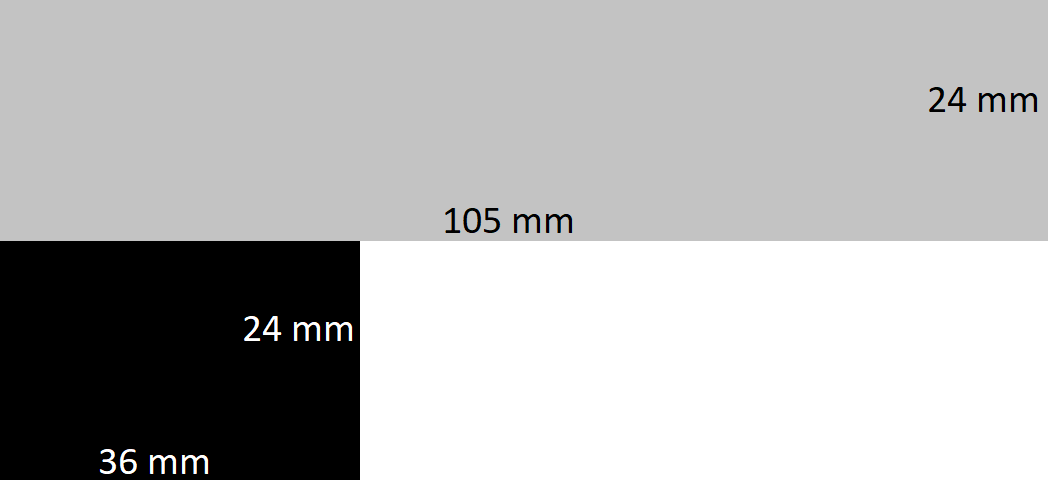
\includegraphics[width=0.7\linewidth]{Images/filmscale.png}
    \caption{A scale illustration to compare a standard $35 \ \text{mm}$ shot (in black with white text) to one of our shots (in grey with black text).}
    \label{fig: film scale}
\end{figure}

The film is held in continuous reels, as shown in figure \ref{fig: reel pic}. Professor David Bailey, the foremost stakeholder or this opportunity, expressed a very strong desire to not the cut the film (keep the reel intact). Not cutting the film introduced challenges because many film scanners can automate the scanning process if a selection of film fits within a certain length. Moreover, cut film is easier to manage when scanning than a continuous reel; a continuous reel must be propped in such a way that it does not roll while also being in the correct orientation for input into the scanner.
\begin{figure}[H]
    \centering
    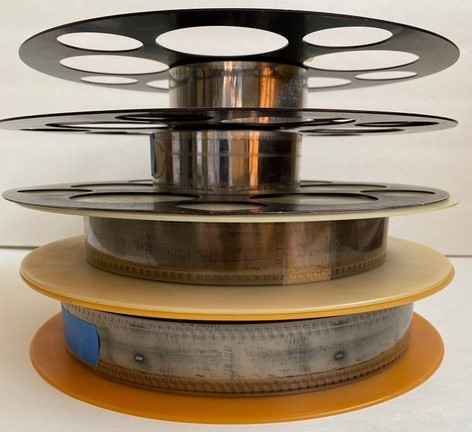
\includegraphics[width=0.7\linewidth]{Images/reelpic.jpg}
    \caption{A photo of our film on a reel, and some empty reels.}
    \label{fig: reel pic}
\end{figure}

Scanning film is time consuming. The 40 photos currently scanned and available to students are at 4800 DPI. The current scanner in the Advanced Lab, an Epson Perfection 4990 Photo, takes about 6 minutes to scan one of our shots at 4800 DPI. Over 200 photos, this comes out to about 20 hours of scanning. Lower DPI, such as 2400, takes less time per shot but produces a less sharp scan. A major challenge of this design opportunity is to reduce this time, or at least develop a procedure to make the scanning process more bearable and comfortable for the operator.

Finally, the film is also delicate, damage to the film in the form of scratches or creases is irreversible. Hence, there was the challenge to reduce any chance of damaging the film.

Scanning the film is ultimately a one time event, once the film is digitized it will not need to be scanned again. Thus, any potential solution should treat time commitments and budgets as one time costs.

\subsection{Final Design}
The selected design for this opportunity includes two main components: the pair of reel stands and the selected scanner. The reel stands are a method to hold the film such that it can be scanned without being cut, while the scanner is obviously necessary to scan and digitize the film.

The overall scanning process involves the preliminary steps of first constructing and loading the reels into the reel stand. Then, the reel stands and film can be placed over the scanner to allow scanning. After these preliminary steps, the scanning process can begin. The user closes the scanner hood, completes a short preview scan, and uses the preview to select the scanning area on the computer. Then the final scan can take place. The final scan takes about 3 minutes to 4 minutes, but the user can leave the scanning set up completely unattended during this time. After the final scan is complete, the scanner hood is lifted, the film is advanced by turning the collection reel, and the scanning process repeats. 

The scanning process takes 4.5 minutes to 5 minutes per shot, and the preliminary steps can take 5 minutes to 15 minutes (however they only need to be done once per reel).

\subsubsection{Reel Stand Design}
Figure \ref{fig: full setup} shows a completely set-up pair pair of reel stands, with a loaded reel. Figure \ref{fig: side profile} is a side profile of a reel stand. Figure \ref{fig: reelsstandsinaction} shows the reel stand being used with the scanner to scan a section of the reel. As shown, the film is pulled across from one reel stand to an initially empty collection reel, with the intermediate film allowed to lay over the scanner. The scanner is closed and scanning commences. The collection reel is then turned slightly to advance the film to the next shot and the process is repeated.
\begin{figure}[htb]
    \centering
    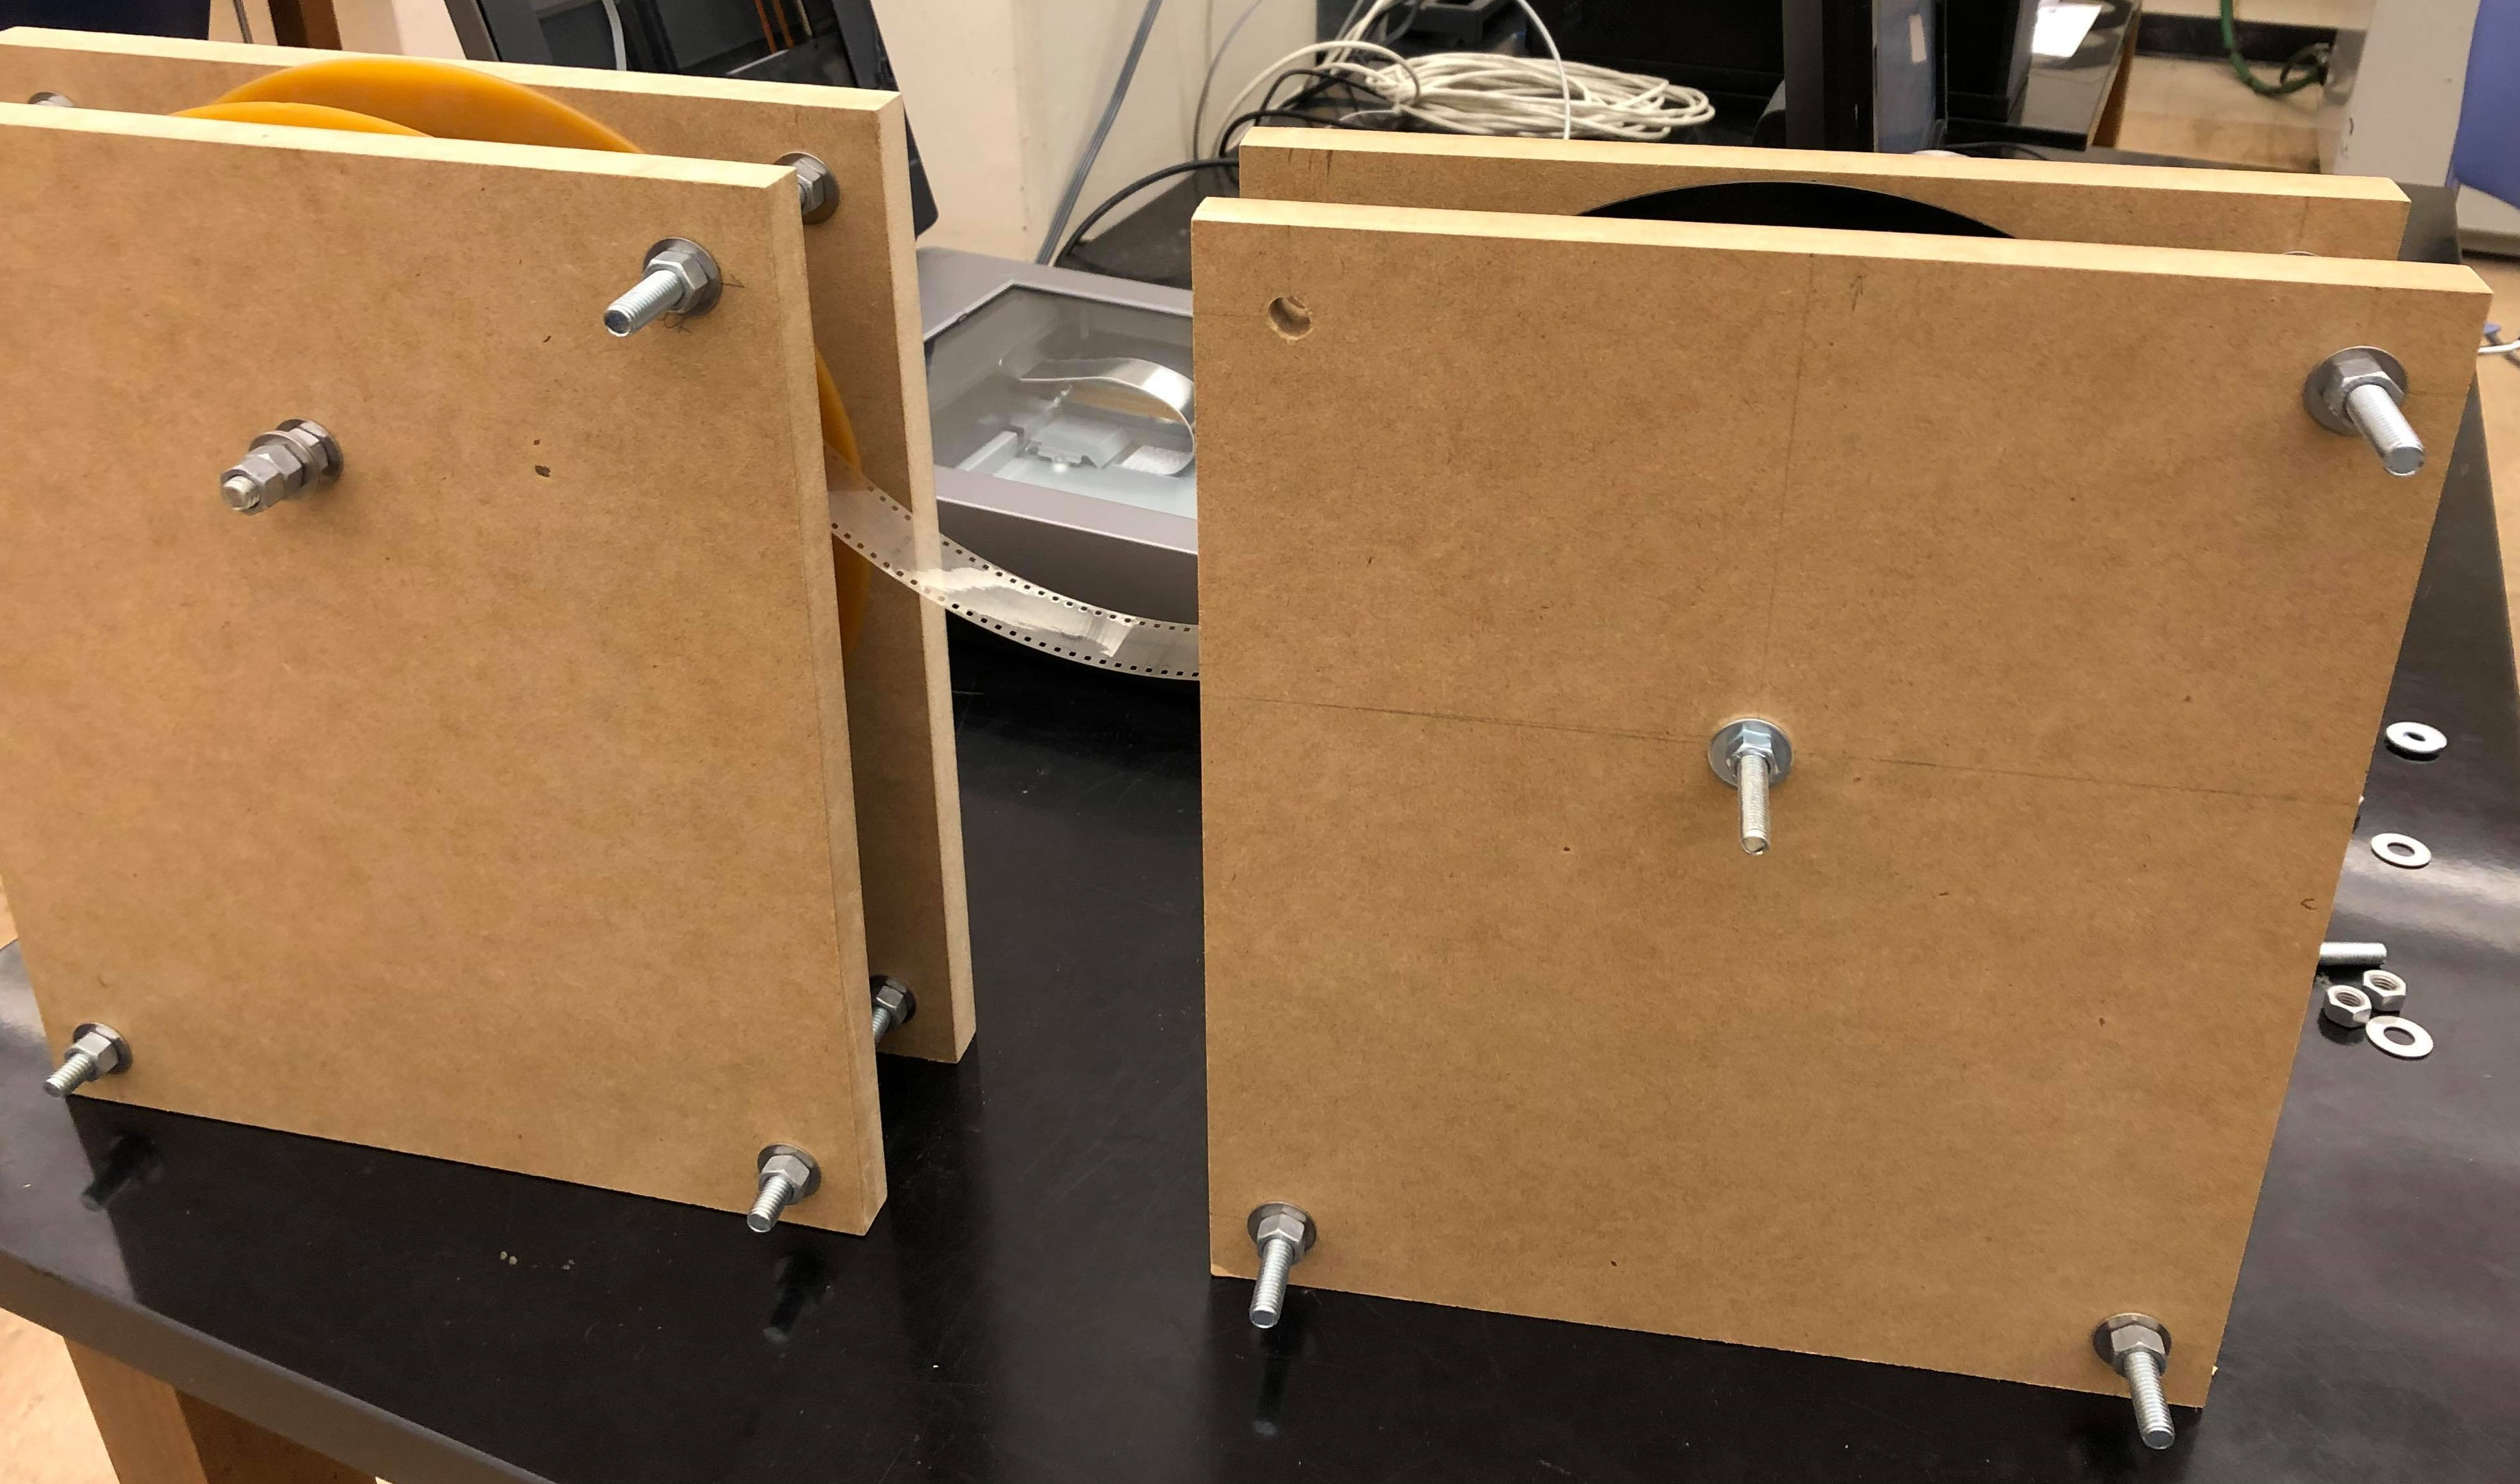
\includegraphics[width=0.7\linewidth]{Images/Reel stand images/setupreelstands.jpg}
    \caption{A completed pair of reel stands, with loaded reel.}
    \label{fig: full setup}
\end{figure}
\begin{figure}[htb]
    \centering
    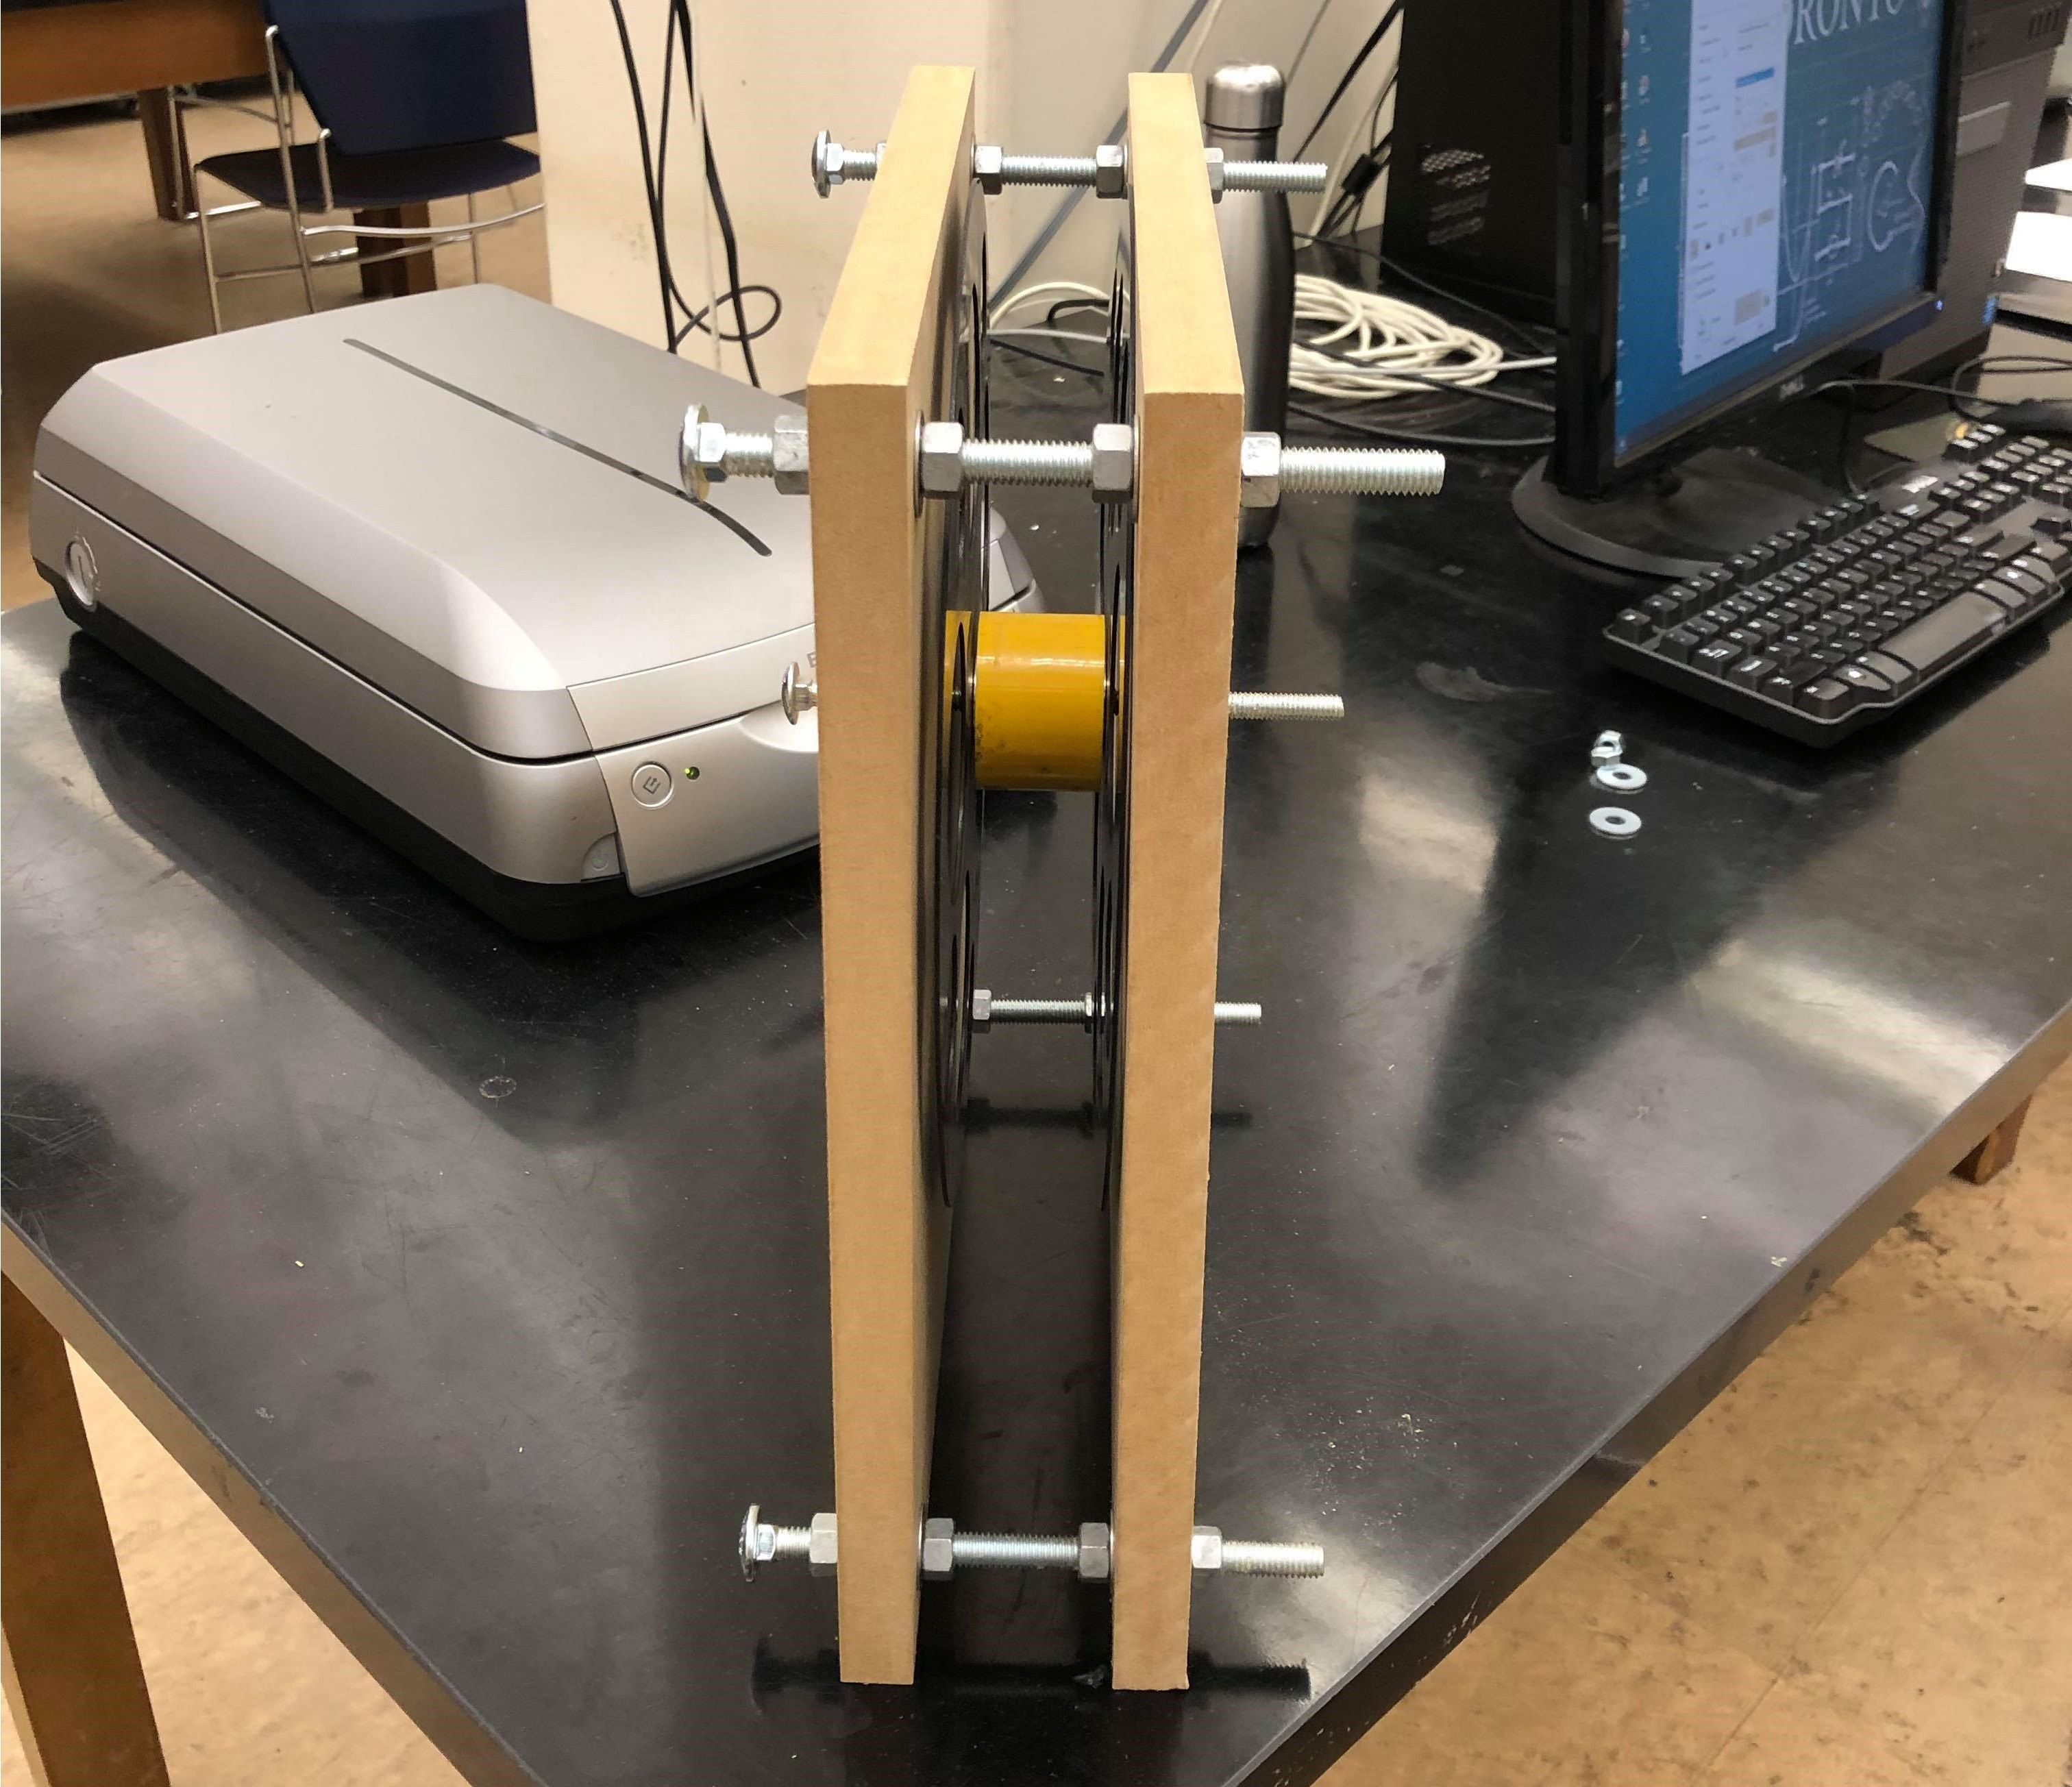
\includegraphics[width=0.7\linewidth]{Images/Reel stand images/reelstanddone.jpg}
    \caption{The side profile of a completed reel stands, with loaded reel.}
    \label{fig: side profile}
\end{figure}
\begin{figure}[htb]
    \centering
    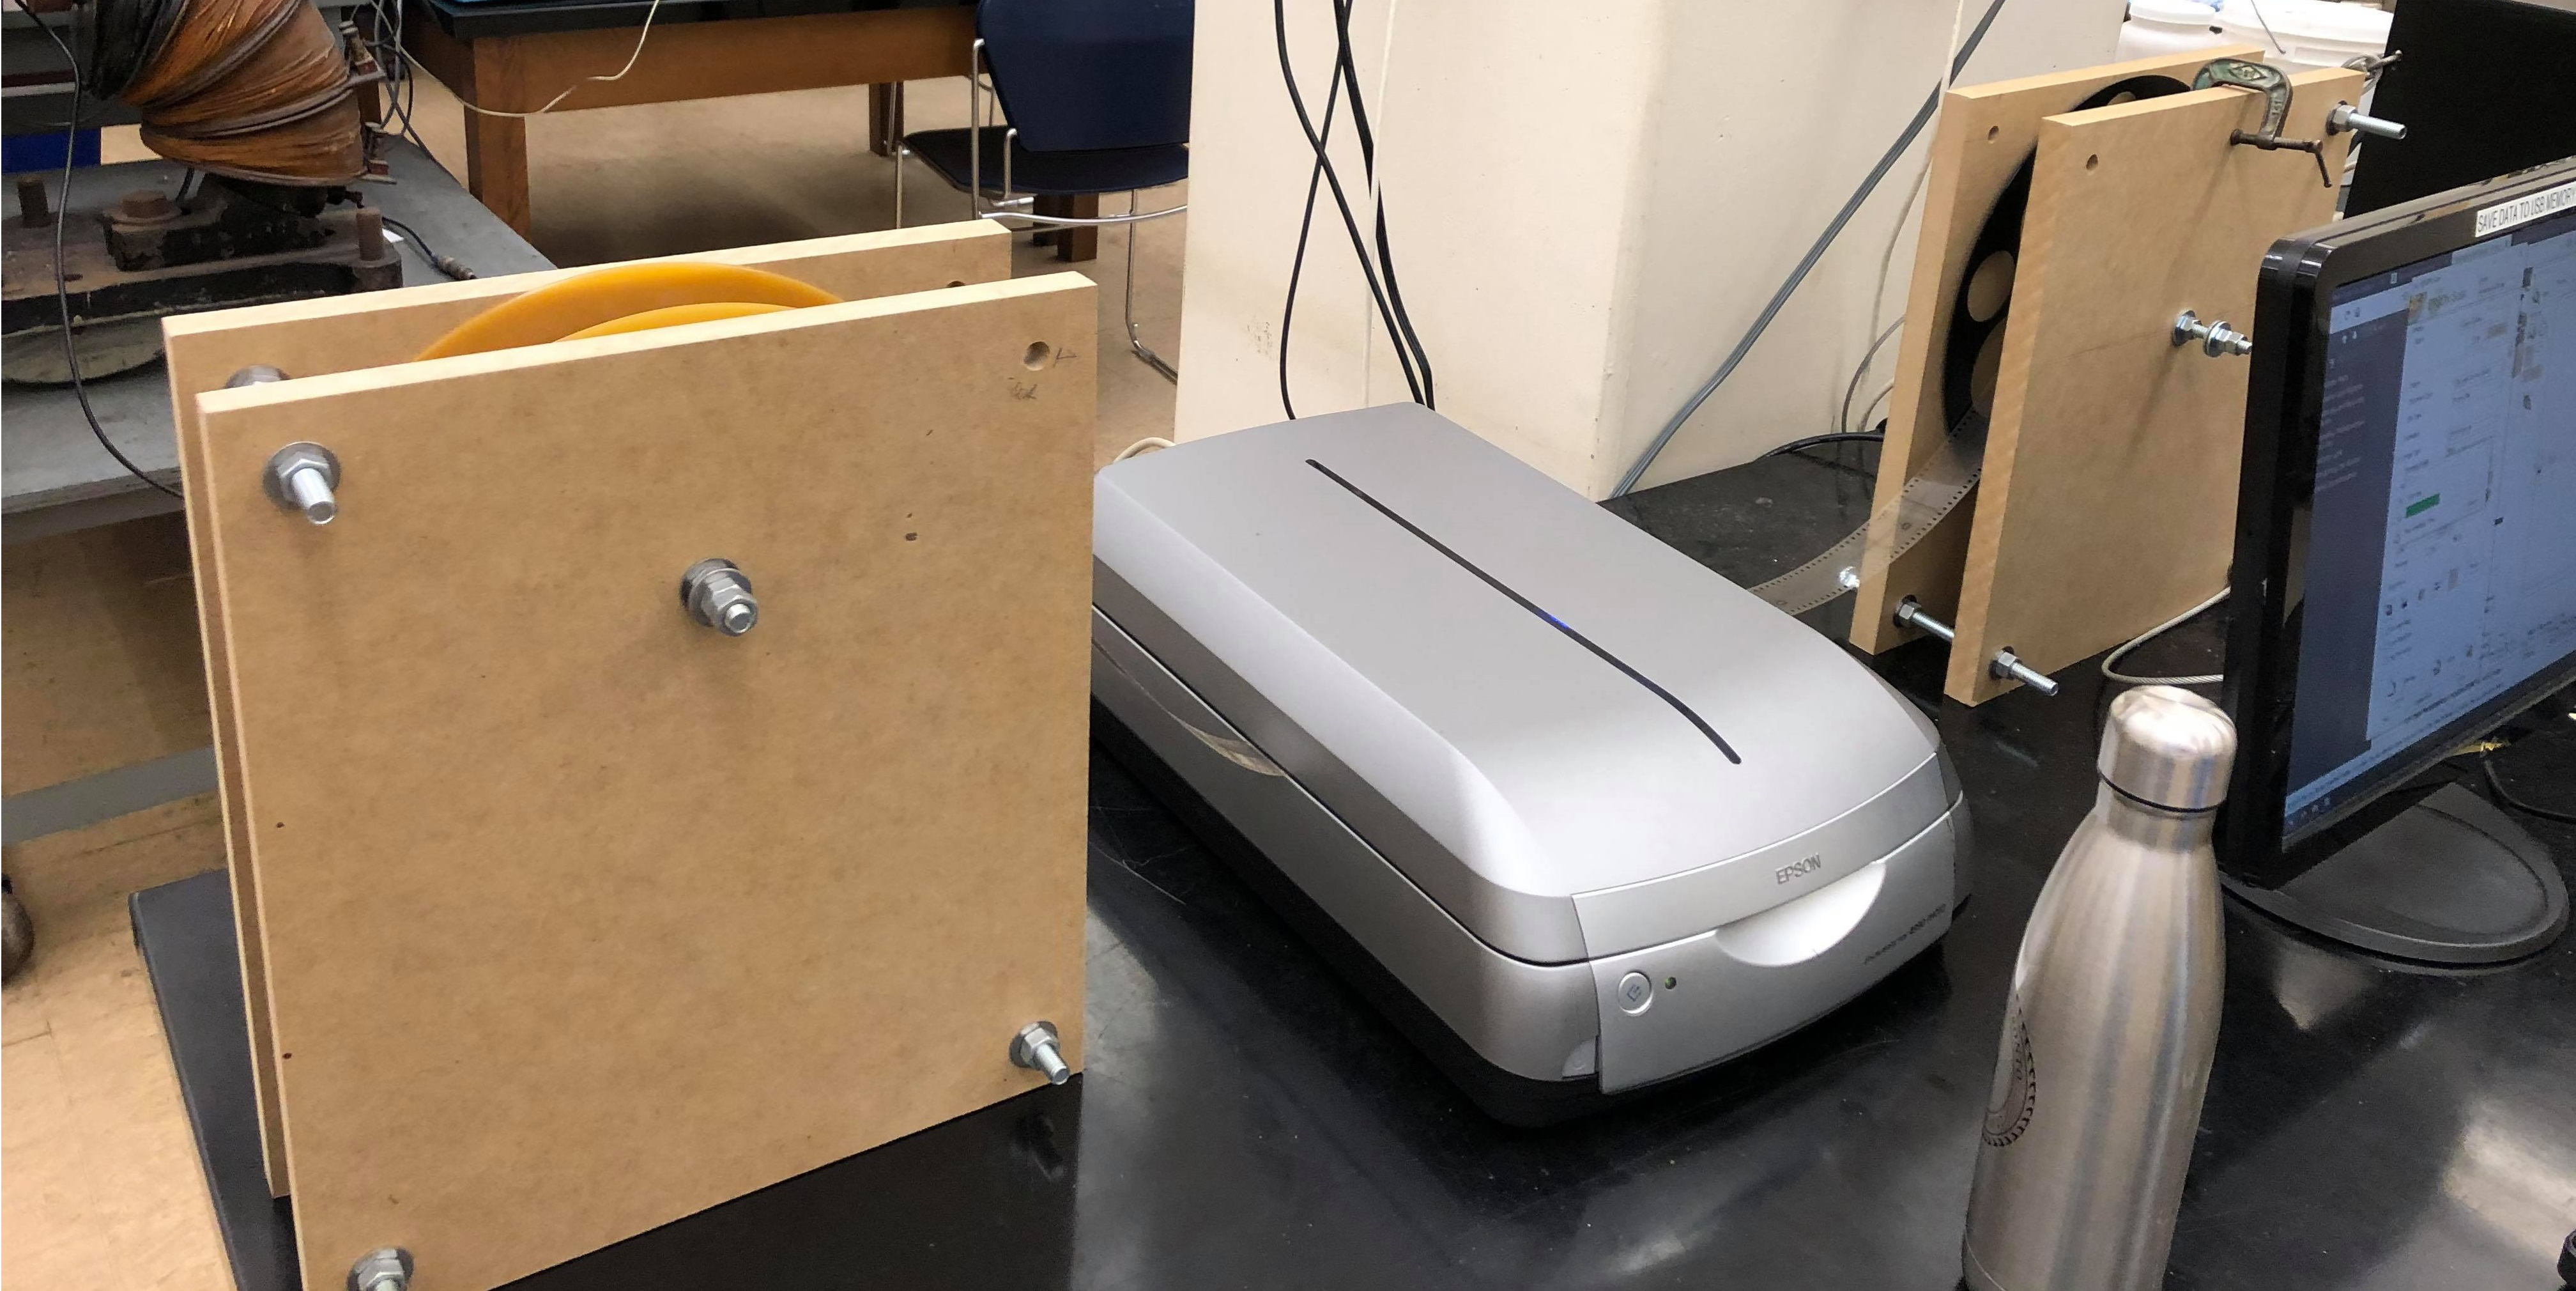
\includegraphics[width=0.7\linewidth]{Images/Reel stand images/reelstandaction.jpg}
    \caption{A completed pair of reel stands, with loaded reel, set-up in a scanner.}
    \label{fig: reelsstandsinaction}
\end{figure}

Each reel stand is comprised of two wood sheets and five screw components. These are shown in figure \ref{fig: reelstanddismantled}. Each screw component is also comprised of several washers and nuts that sandwich the wooden sheets.
\begin{figure}[H]
    \centering
    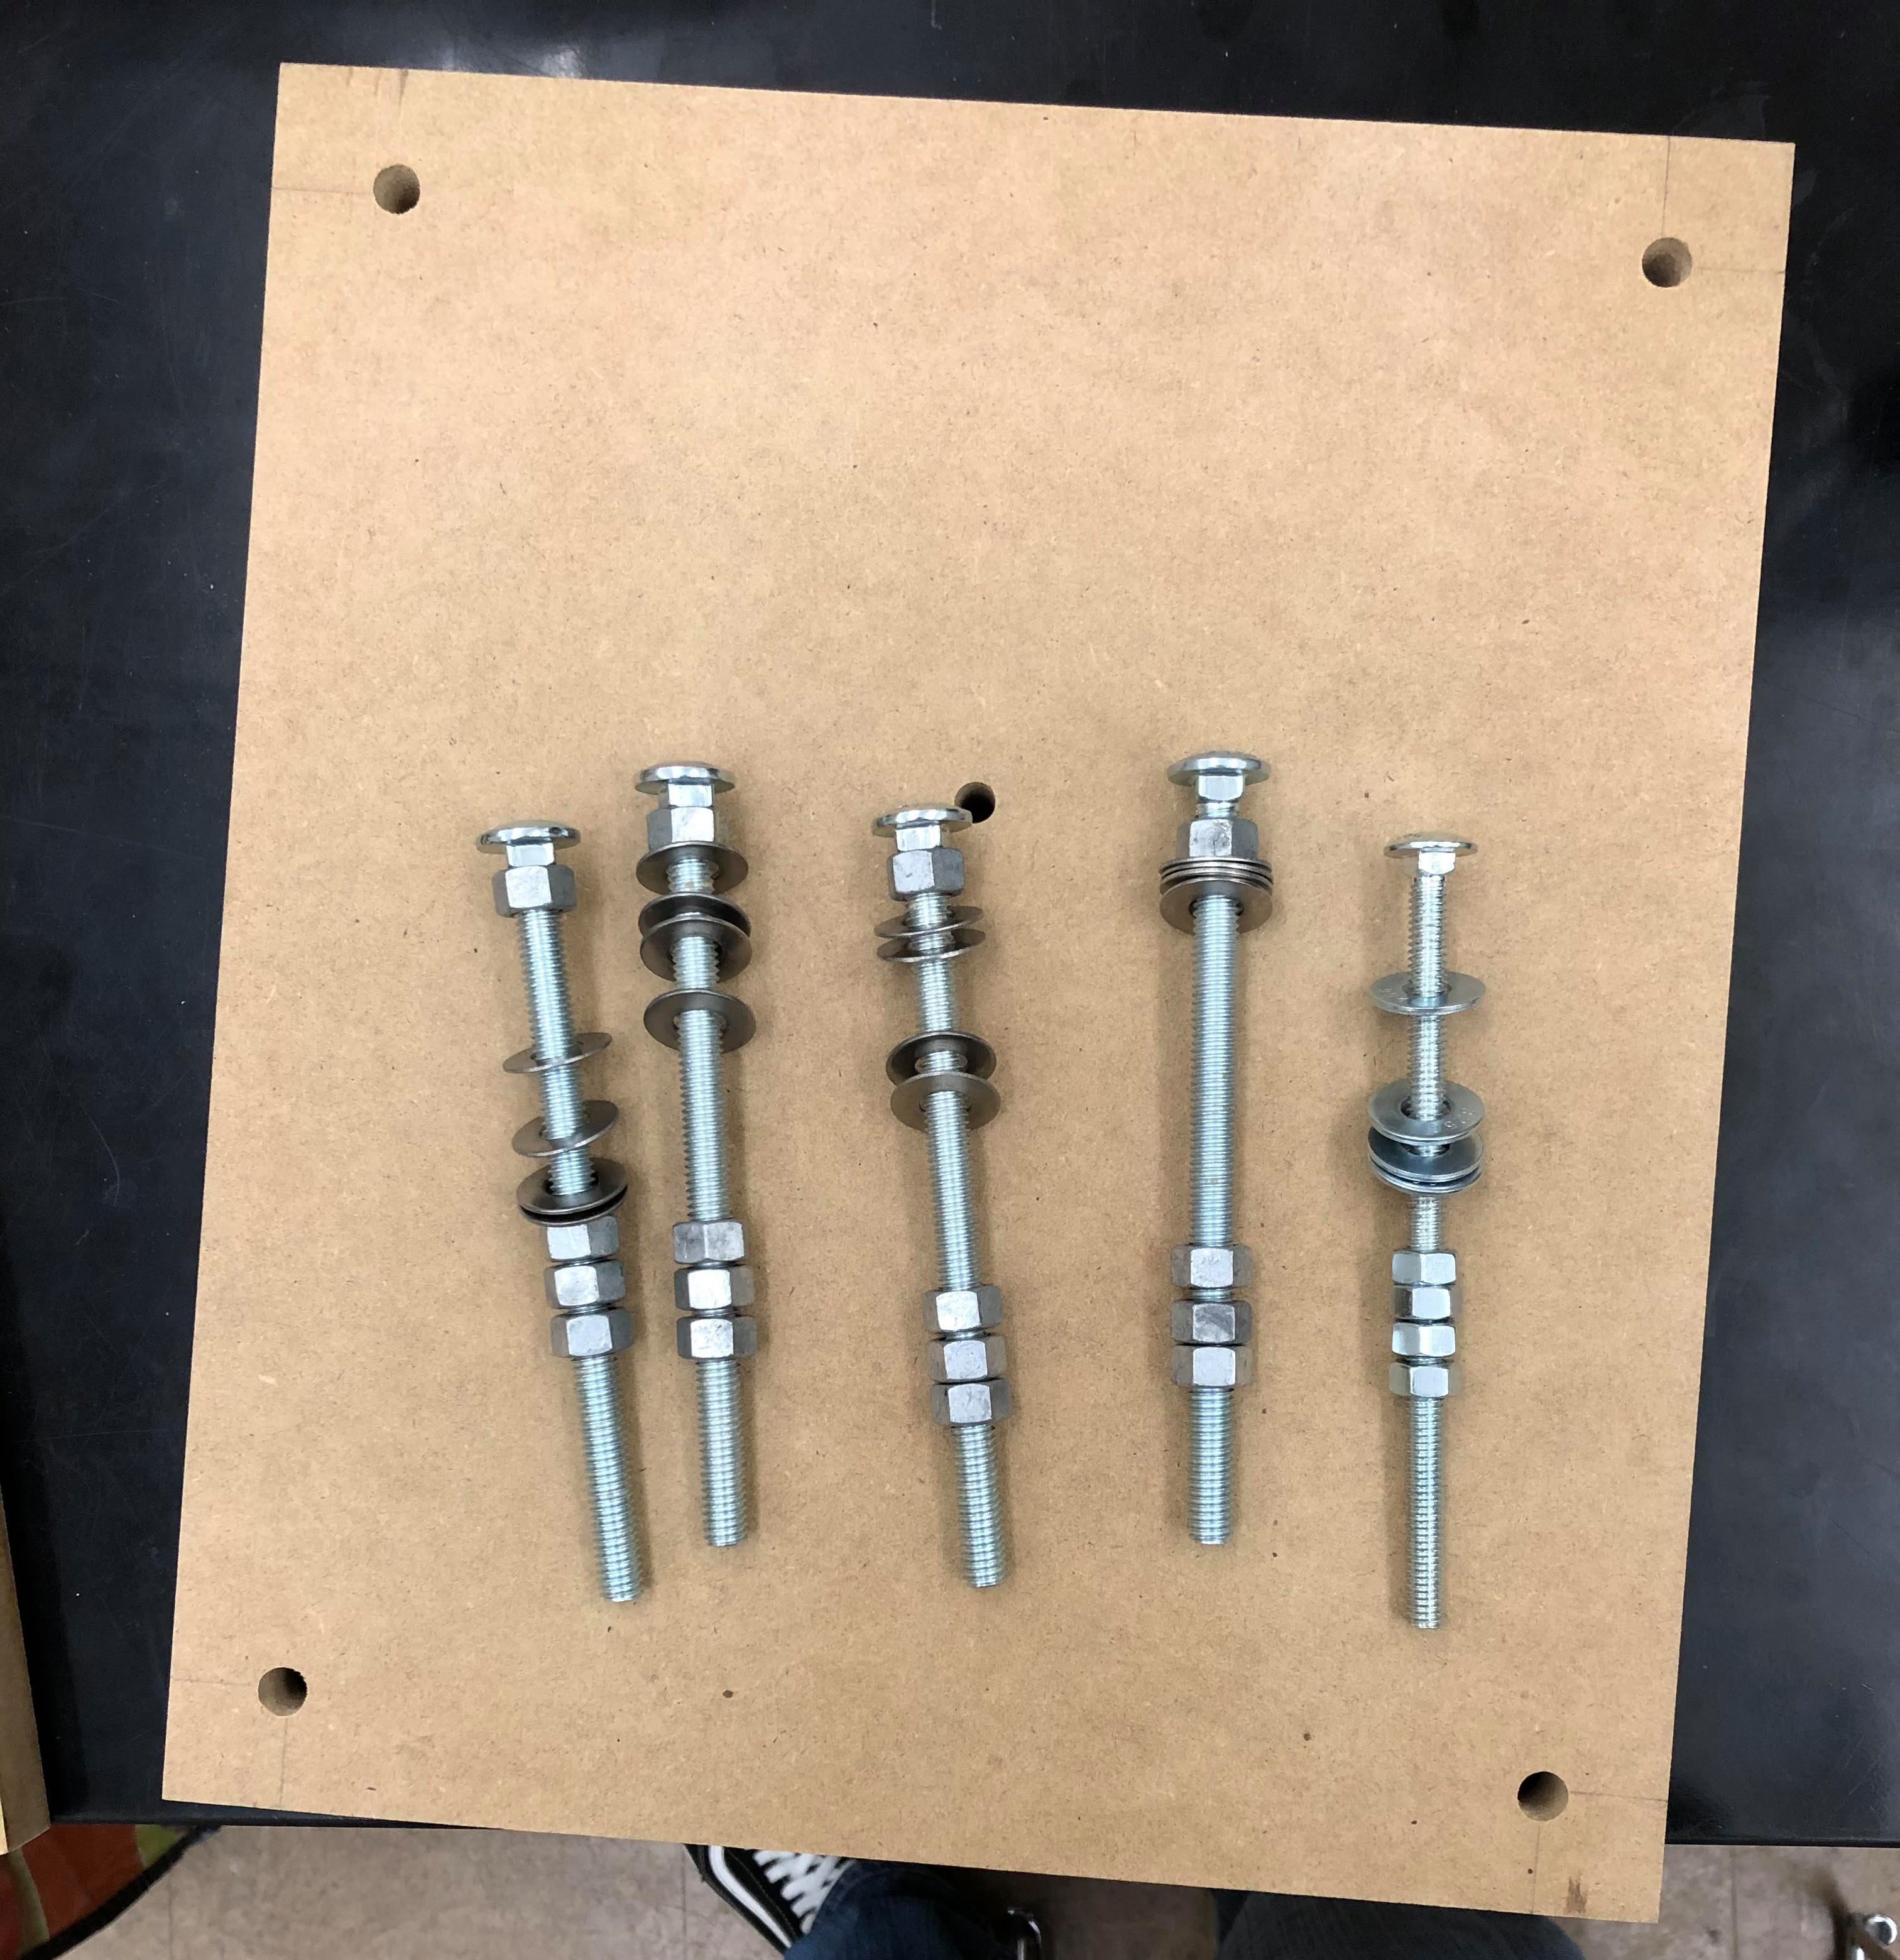
\includegraphics[width=0.7\linewidth]{Images/Reel stand images/reelstanddismantled.jpg}
    \caption{A dismantled reel stand.}
    \label{fig: reelstanddismantled}
\end{figure}

To construct a reel stand, four screw components are first attached to one wood sheet in a nut-washer-woodsheet-washer-nut sequence, as shown in figure \ref{fig: reelstand4screws}. Then, the fifth screw component, the axle screw, can be inserted into the wood sheet and a reel can be placed on to it, as shown in figure \ref{fig: reelstandscrewsandreel}. Notice that the axle screw does not have washers or nuts on the inside of the wood sheet, this is to create a tight space between the wood sheets to eliminate the reel from moving across the axle. Finally, the second wood sheet is attached by repeating the nut and washer arrangement for the screw components, as shown in figure \ref{fig: side profile}. In figure \ref{fig: full setup} you will notice that the one of the top corners of one of the reel stands is missing a screw component; indeed that component is optional and can be removed to limit the film from touching any undesirable surfaces. The reel stand can be entirely constructed with one's hands, no tools at all are needed as ``finger tightening" makes the stand sufficiently rigid.
\begin{figure}[H]
    \centering
    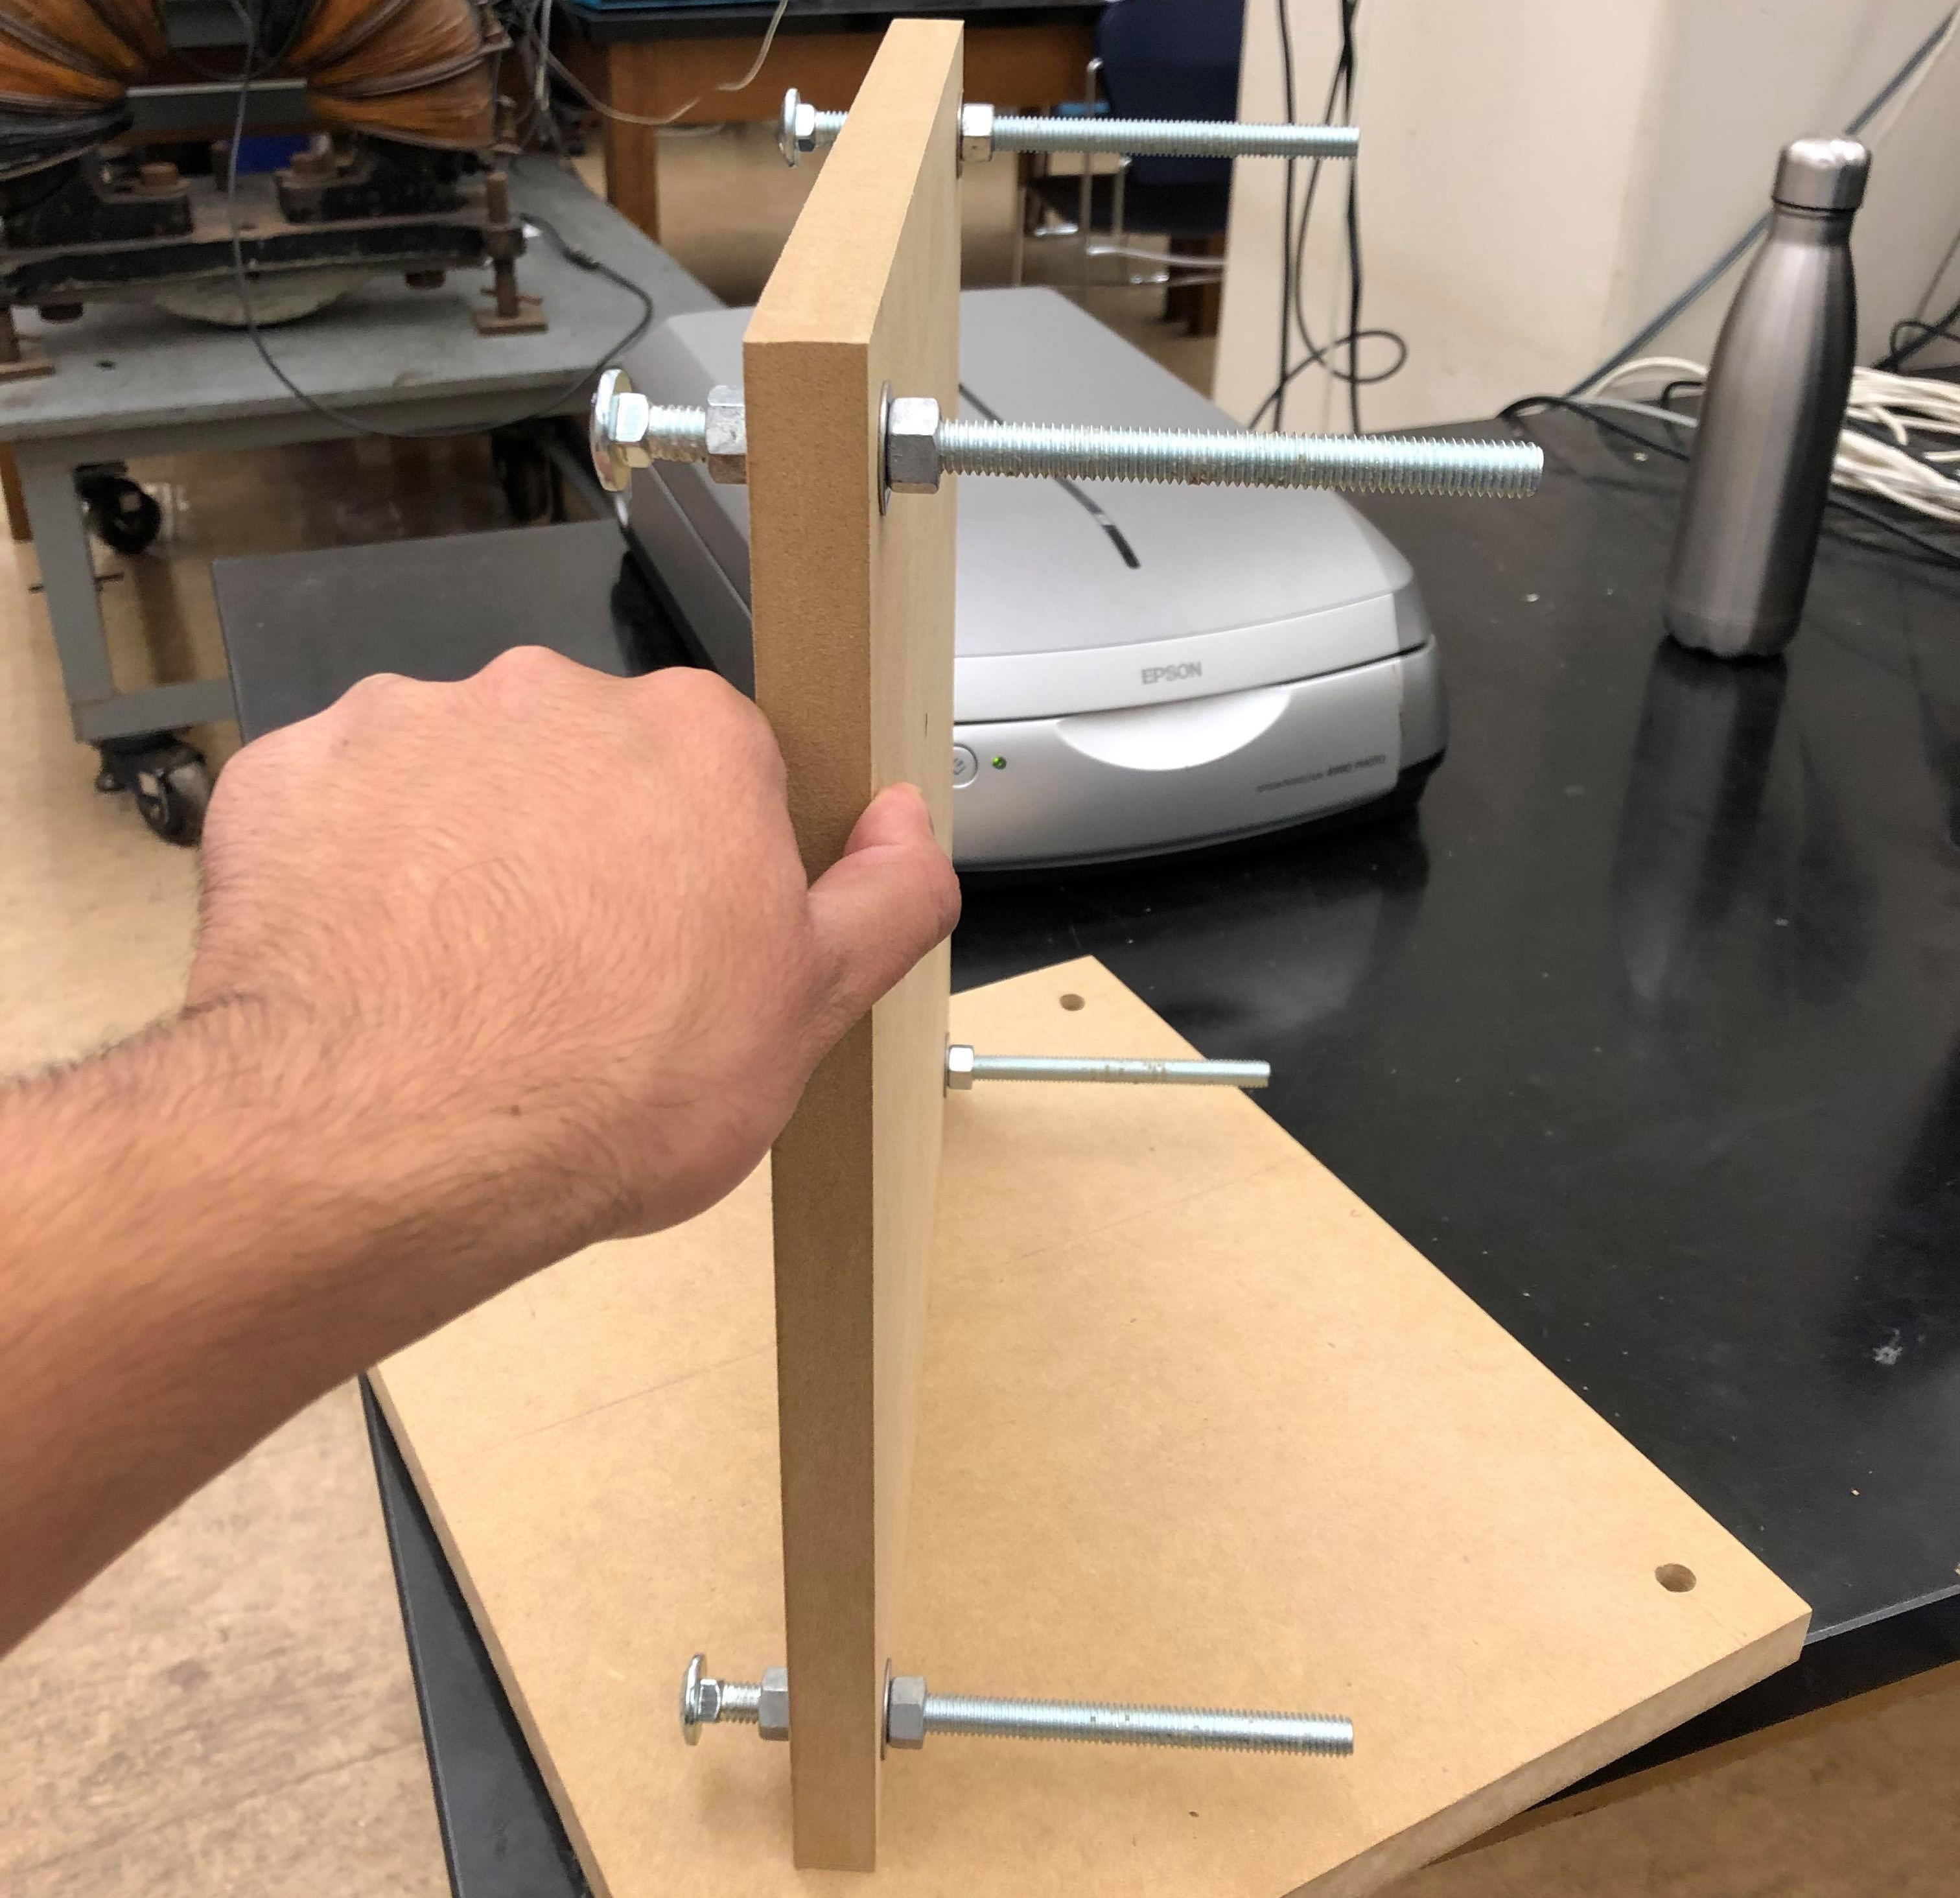
\includegraphics[width=0.7\linewidth]{Images/Reel stand images/reelstand4screws.jpg}
    \caption{A partially built reel stand, with four attached screw components to one wood sheet.}
    \label{fig: reelstand4screws}
\end{figure}
\begin{figure}[H]
    \centering
    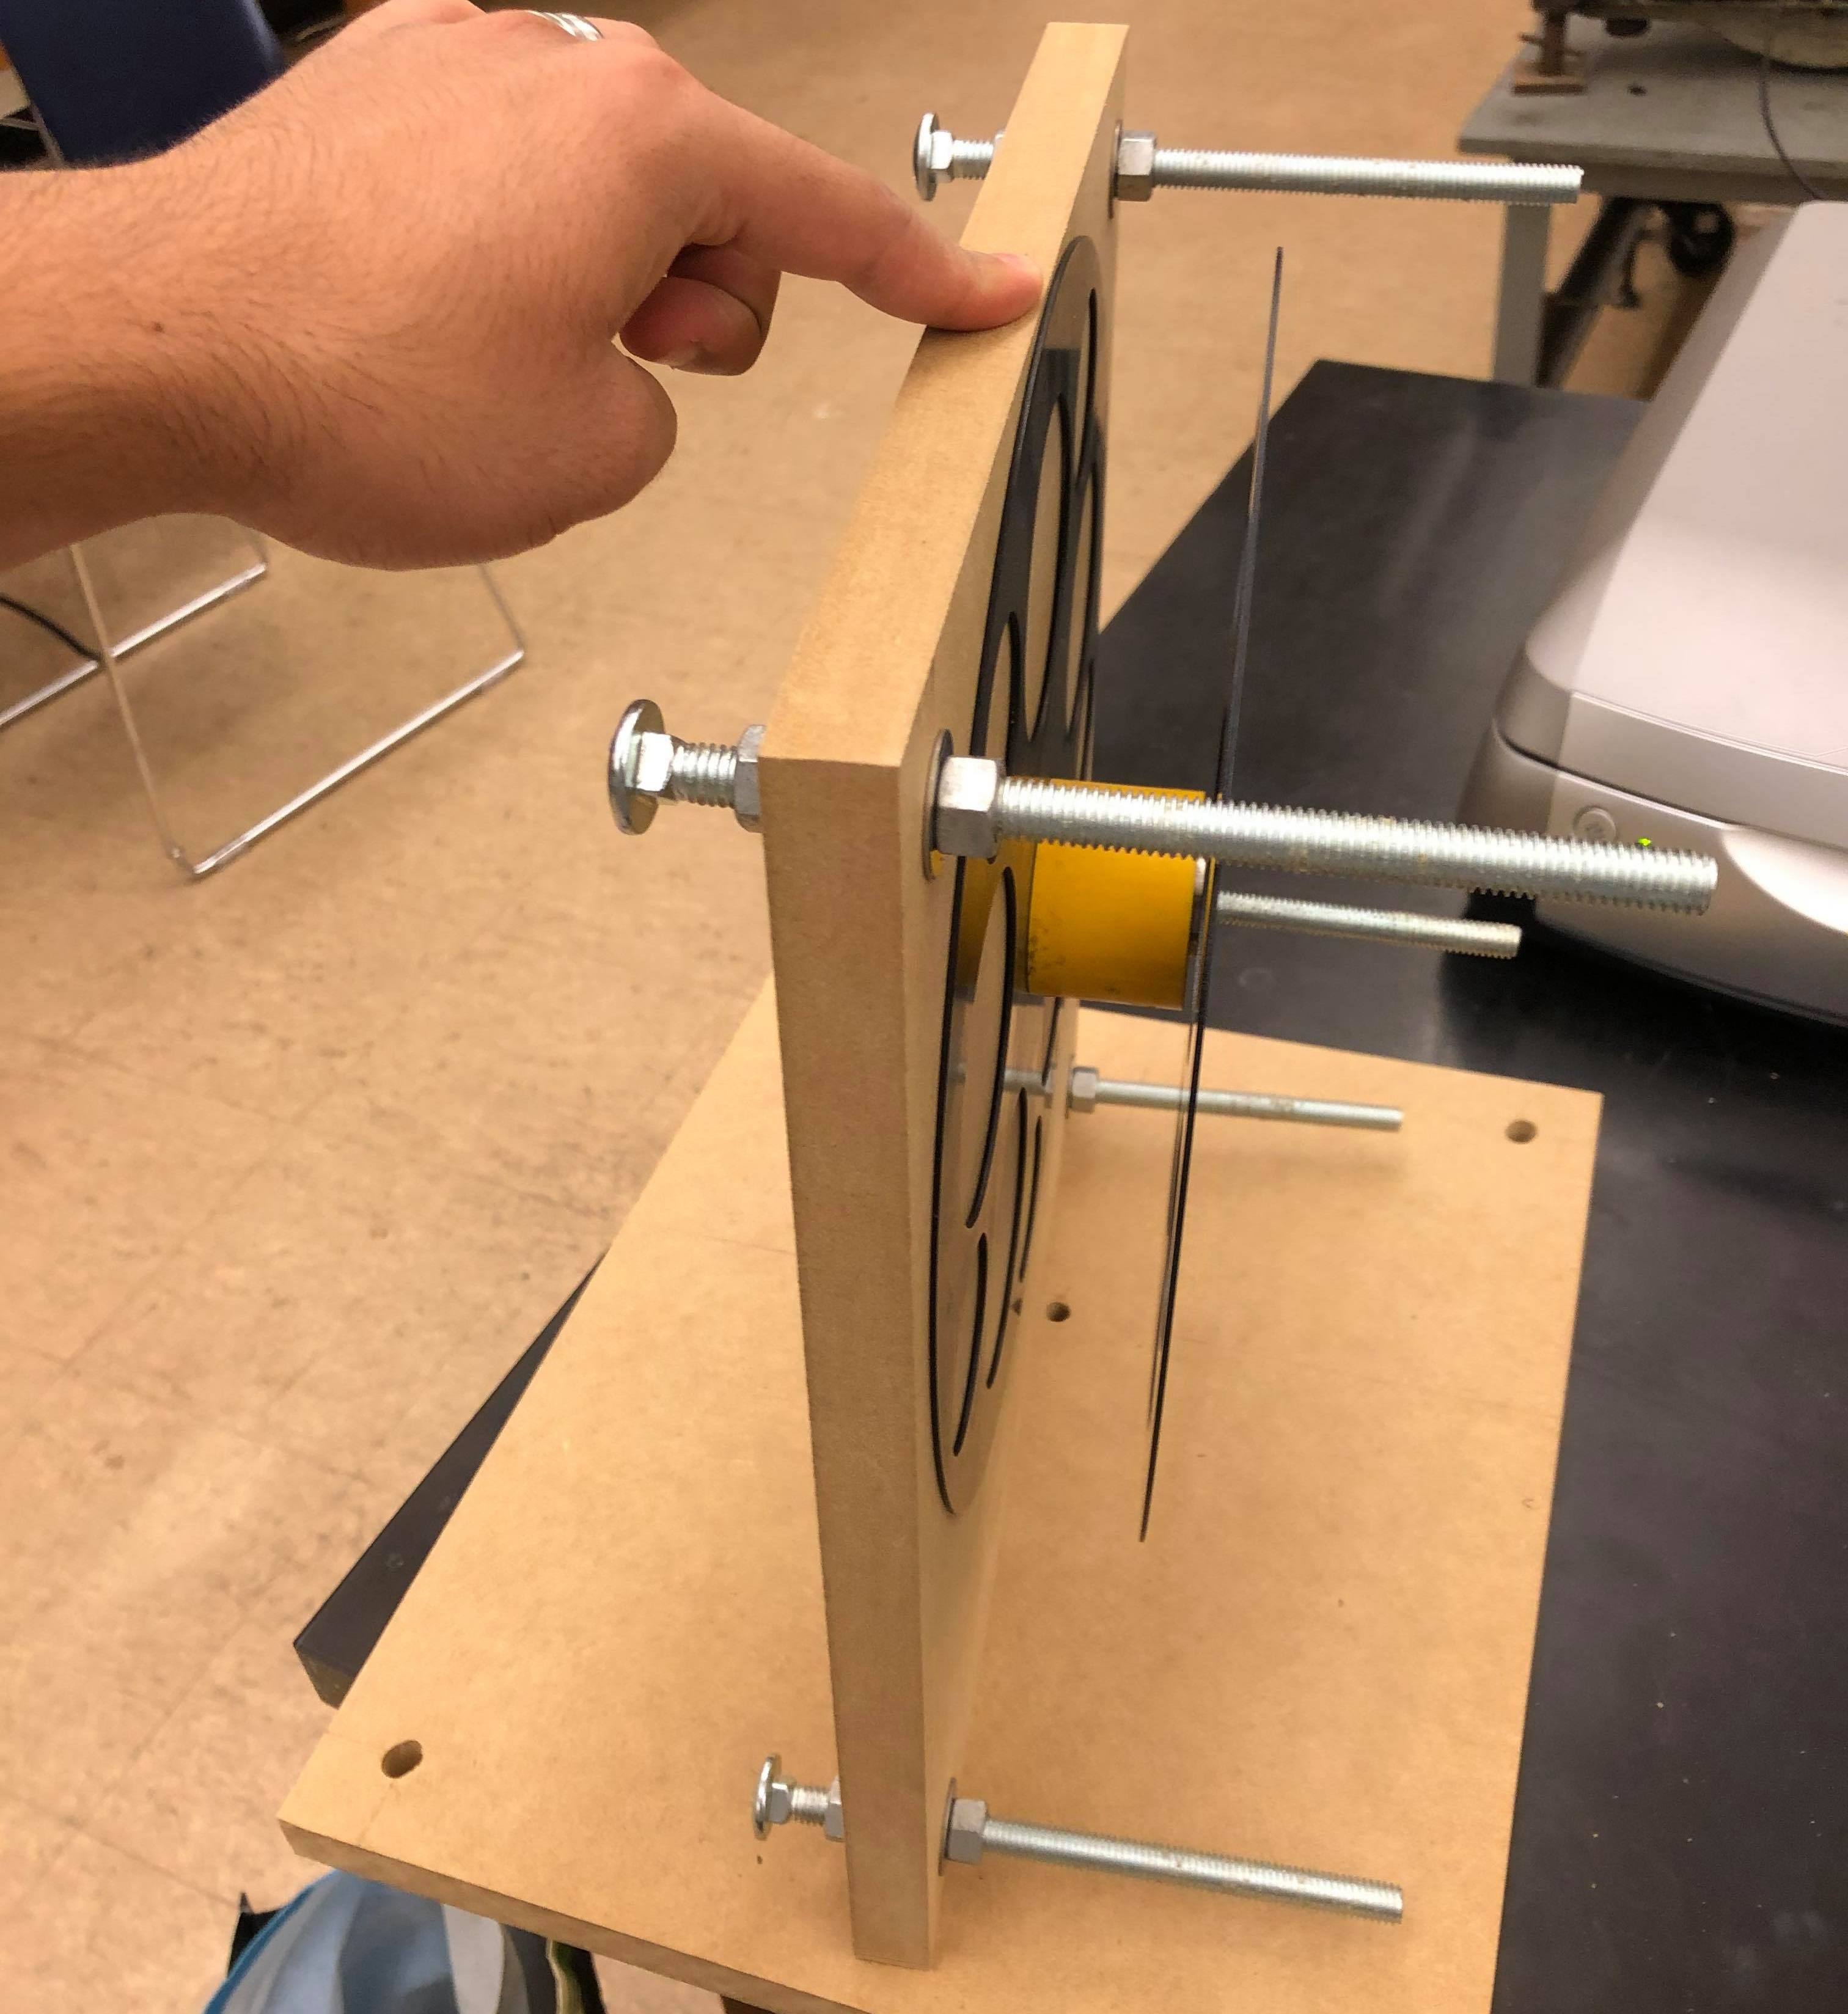
\includegraphics[width=0.7\linewidth]{Images/Reel stand images/reelstadnscrewsandreel.jpg}
    \caption{A partially built reel stand, with four attached screw components to one wood sheet and a loaded reel.}
    \label{fig: reelstandscrewsandreel}
\end{figure}

Each wood sheet has dimensions $12 \ \text{inches} \times 14 \ \text{inches} \times \frac{3}{4} \ \text{inches}$. These dimensions were selected to be as compact as possible, while still allowing a $1 \ \text{inch}$ horizontal buffer on each side, a $1 \ \text{inch}$ vertical buffer on the top, and a $2 \ \text{inches}$ vertical buffer on the bottom of the wood sheet. These buffers allowed the screw holes to be drilled far enough into the wood sheet that any potential splitting could be eliminated. Moreover, the $2 \ \text{inches}$ vertical buffer allowed the reel stands to lift the reels slightly higher so they could be more level with the scanners, and lessen the chances of the film becoming contaminated by touching a table.

The reel stands have a variable width depending on the width of the loaded reel, varying form $9 \ \text{cm}$ to $11 \ \text{cm}$. These width were more than sufficiently stable in our tests; the stand never fell over or wobbled except from extremely deliberate knocking. The stability of the stands also benefits from their overall weight (about $7$ pounds each) and rigid construction due to the friction of washers and nuts on each side of each wood sheet.

The screws all have  a length of  $6 \ \text{inches}$. The corner screws have a diameter of have a diameter of $\frac{3}{8} \ \text{inches}$, two axles screws also have this diameter, while two other axle screws have a diameter of $8 \ \text{millimeters}$. The varying axle screw diameters are to account for the different hole sizes the different reels have.

There is an optional clamp that can be used with the collection reel for the first few shots, as shown in figure \ref{fig: reelsstandsinaction}. The clamp simply holds the reel in place for the first two or three shots as the reel tends to unroll before enough film is advanced to wind around the reel at least once. In our testing, we generally only needed the clamp for the first two shots, after which there was enough film to wind around the reel.

One design theme of the reel stands is modularity, they were designed so that they can be dismantled and put together with ease and be stored compactly. Modularity also allowed us to design the reel stands using basic materials (very common screws and bolts and wood sheets) and basic techniques and tools (just some drills and saws). One way modularity is realized in the design is in the axle screws, there is a choice of which axle screw to use depending on the reel used; in figure \ref{fig: full setup} the left reel stand uses a smaller axle than the right.

The total cost of the reel stands was $\$40$ each, however this was because wood, bolts, and washers were not available in the small quantities required. A more economically scaled cost is around $\$25$ each. Construction time for the reel stands was 4 hours total, requiring an electric circular saw and a hand drill.

\subsubsection{The Selected Scanner}
The selected scanner for this design opportunity was the Epson Perfection 4990 Photo already present in the Advanced Lab, as seen in figure \ref{fig: reelsstandsinaction}. The scanner meets the minimum image quality constraint of 4800 DPI, and provides sufficient speed to allow a fast but comfortable scanning experience. While scanners with somewhat faster scanning times were available for purchase, they did not provide better image quality and thus their purchase was unjustifiable. 

\subsection{Objectives, Metrics, Constraints, and Our Design's Performance}
\subsubsection{DFX Considerations}\label{dfx}
For this design opportunity, many of the DFX consideration are effectively objectives as well. Nonetheless, we determined several overall design goals and consideration.

Firstly, we designed for speed. Ultimately, the speed of the overall scanning process was limited by the scanning speed of the scanners. However, there are several areas where we considered speed. For example, the scanner's settings are fast and easy to set for each scanning session, or that we should scan in such a way that post-scan editing is as minimal and fast as possible.

Secondly, we will design for ease. Many of the design consideration for an easy and comfortable process overlap with those of a fast process. However, there are still some unique considerations. For example, the scan operator should not have to continuously stop the film reel from rolling, or be standing for the whole process.

Finally, we will design for quality, in particular, the quality of the scans. We have some preferences and constraints regarding the quality of the scans, and we will design the process to meet them.

\subsubsection{Fast Scanning Process} \label{subsubsection: objective fastscanningprocess}
We have an objective to make the scanning process as fast as possible. As mentioned in section \ref{dfx} we are ultimately limited by the scanning speed of scanners, but we will try to minimize the overall scanning process time. Time sensitive parts of the scanning process include: powering and warming up the scanner, loading the film, setting the scanner to scan the film, the actual scanning time, post-scan editing, advancing the film to the next photo, and storing the film.

\paragraph{Metric: Set-up Time}
\begin{itemize}
    \item Description: This metric measures the time taken to begin the scanning process, on average, lower is better. This includes powering on the scanner and computer, and setting up any method to hold the reel.
    \item Measurement: Seconds or minutes; begin measuring when scanner is powered on, end measuring when the first scan is ready to be performed.
    \item Final performance: 5 minutes to 15 minutes, only needed once per reel. Typical case is 8 minutes. This metric adequately satisfied our and our stakeholders' desires for a fast set-up time.
\end{itemize}

\paragraph{Metric: Scan Time Per Photo} 
\begin{itemize}
    \item Description: This metric measures the time taken to scan one photo, on average, lower is better. This includes advancing the film from the last photo to the current photo, preparing the scan, and the time the scanner takes to actually scan the photo.
    \item Measurement: Seconds or minutes; begin measuring then advance the film to the current photo, end measuring when the photo is completely scanned.
    \item Final performance: 4.5 minutes to 5 minutes. This metric adequately satisfied our and our stakeholders' desires for a fast scanning time.
\end{itemize}

\paragraph{Metric: Editing Time Per Photo} 
\begin{itemize}
    \item Description: This metric measures the time taken to edit one scan, on average, lower is better. This includes any cropping or color correction done to a photo after it has been scanned.
    \item Measurement: Seconds or minutes; begin measuring once the editing process begins, end measuring once editing is complete.
    \item Final performance: 10 seconds to 30 seconds. This metric adequately satisfied our and our stakeholders' desires for a fast editing time per photo.
\end{itemize}

\paragraph{Metric: Total Scanning and Editing Time Per Photo} 
\begin{itemize}
    \item Description: This metric measures the time taken to edit and scan a single photo, on average, lower is better. In other words, this metric measures how long it takes to fully prepare one photo for use in the HEP experiment. 
    \item Measurement: Seconds or minutes; sum of scan time per photo and editing time per photo.
    \item Final performance: 4.5 minutes to 5 minutes. This metric adequately satisfied our and our stakeholders' desires for a fast total scanning and editing time. This metric is effectively the same as Scan Time Per Photo because ``editing" (preview scan and crop) is done after advancing the film but before scanning the film.
\end{itemize}

\subsubsection{Easy/Comfortable Scanning Process} \label{obj easy scan proc}
We have an objective to make the scanning process and easy and as comfortable as possible. While it is difficult to quantify comfort and and ease, we will use leisure time available to the scan operator per photo or scan to measure comfort.

\paragraph{Metric: Leisure Time Per Photo}
\begin{itemize}
    \item Description: This metric measures the time available to available to the operator to occupy themselves with another task, per scan. Higher is better for the same scan time per photo (see section \ref{subsubsection: objective fastscanningprocess}).
    \item Measurement: Seconds or minutes; begin measuring once the operator can leave the scanner completely unattended, end measuring once the scan is complete.
    \item Final performance: 3 minutes to 4 minutes, typical case is 3 minutes. This metric adequately satisfied our and our stakeholders' desires for a comfortable scanning process; scan operators will have a comfortable time to watch videos, read books, or work on homework while waiting for scans to complete.
\end{itemize}

\subsubsection{High Scan Quality} \label{obj high scan quality}
We have an objective to match at least the scan quality of the current photos available to HEP students, 4800 DPI. We will also try to improve scan quality in terms of contrast and sharpness as some of the extensions the HEP experiment will see from software improvement and expansion depend on improved scan quality in these areas.

\paragraph{Constraint: Minimum 4800 DPI for Newly Scanned Photos}
\begin{itemize}
    \item Newly scanned photos must be at least 4800 DPI to match the quality of the scans currently available to HEP students.
    \item Final performance: constraint met, all scans are at 4800 DPI.
\end{itemize}

\subsubsection{Avoid Cutting Film}
Finally, we have an objective to avoid cutting the film reel. Professor Bailey has greatly expressed the desire to avoid cutting the film reel (see section \ref{profbaileyscanning}). This is not a constraint however, as Professor Bailey has described some conditions under which he would be more comfortable with cutting the film, and film has been cut in the past by other Capstone groups working on the HEP experiment.

Our final design does not require any film to be cut, so we definitely satisfy Professor Bailey's objective.

\subsection{Stakeholders}
This section analyzes each stakeholders in relation to the design opportunity, the preferences they have expressed, how and if we satisfied their preferences, and our interactions with them thus far.

\subsubsection{Professor David Bailey} \label{profbaileyscanning}
Professor Bailey is the foremost stakeholder. He is the coordinator of the Advanced Lab, and thus he is in control of the film, the currently owned scanner, and the budget for the new scanner. As the coordinator of the Advanced Lab he will have ultimate control over design decisions, such as which scanner to use or purchase, but it is our role to inform him to the best of our abilities.

Professor Bailey has expressed several preferences that inform our design decisions and objectives. Firstly, Professor Bailey has strongly expressed a desire to keep the film reel intact. If the film is to be cut, Professor Bailey would like the film to be cut in the Advanced Lab rather than by a local professional service. Our design does not need any film to be cut, so we have satisfied his request. Secondly, Professor Bailey would like the resolution and sharpness of the new scans to match that of the 40 scans already available in the HEP experiment; this corresponds to 4800 DPI. Our selected scanner and scanner process meets the 4800 DPI minimum. Finally, Professor Bailey would like the scanning process to be as fast and comfortable as possible for the scan operator. Professor Bailey has envisioned a process that is either so fast that the scan operator will be fully occupied in scanning all the film for a short period of time, or a slower process where the scan operator can comfortably spend time watching a video or reading a book while they wait for scans to finish. Our design meets the second vision, where the scans require minimal participation from the scan operator so that they can occupy themselves with something else while scans are completed. 

We have had very regular contact with Professor Bailey, including several emails a week and a weekly 30-60 minute meeting.

\subsubsection{Scan Operators} \label{scanopsscanning}
Scan operators are significant stakeholders, they are the people who will actually use the developed procedure to scan the roughly 200 photos. Scan operators will likely be the designers (Ruchir and Anas) or a summer intern at the Advanced Lab.

We primarily used ourselves and Professor Bailey to proxy the scan operators. Hence, we have developed several preferences that a scan operator would like. Firstly, the total scanning process should be as fast as possible. This includes the time it takes to scan each shot, set-up the scanner, store and orient the film reel, and any post editing applied to the scans (such as cropping or contrast corrections). The time reduction in scanning is limited by the speed of the scanners, so the second preference is to make the scanning process as comfortable as possible. An acceptable hypothetical situation would involve the operator watching a video or reading a book while they wait for a scan to finish, adjusting the scanner for the next photo, then returning to their video or book. Indeed, the final design meets this hypothetical situation as advancing the film and preparing a scan requires minimal participation from the scan operator, and they can spend the scanning time occupied with something else.

So far, regular internal discussion between the designers and meetings with Professor Bailey have been a proxy for interaction with the scan operator.

\subsubsection{HEP Student Experimenters}
HEP student experimenters are important stakeholders because they will be using the scans for their experiment.

Both designers were HEP student experimenters in the past, so we have used our own experiences as proxy. Moreover, Professor Bailey in his experience as the Advance Lab coordinator has interacted with many HEP student experimenters, so he has helped support our proxy. The only real preferences HEP students have in regards to scanning is that the quality of the scans should be good enough to use the current Traxis software and any additional features we add to it. This preference is met by the 4800 DPI minimum that Professor Bailey has expressed, and is indeed met by our final design.

As with the scan operators, regular internal discussion between the designers and meetings with Professor Bailey have been a proxy for interaction with HEP student experimenters.

\subsubsection{Other Stakeholders}
Other stakeholders for this design opportunity include the supervising professors for the HEP experiment and the Advanced Lab teaching assistants who act as supporting demonstrators. The preferences of these stakeholders are met by the preferences of Professor Bailey, the scan operators, and student experimenters' preferences so separate analysis is not needed.

\subsection{Reel Stands: Previous Designs and Design Decisions}
The basic requirements for a reel stand implied many potential designs. All that a reel stand necessitated was some method to hold the film reel without constant supervision of the scan operator. Such a method must stop the film reel from rolling, eject the film in such a way that it can be scanned by the scanner, and be able to advance the film.

A valid reel stand design should take less time to construct than it takes to scan  all the film, so under 20 hours. If the reel stand takes longer to construct, one should obviously instead use that time to simply scan the film.

Figure \ref{fig: whole set up} shows the initial reel stand design. In the illustration, the first film stand holds the film that has not yet been scanned while the second reel holds the scanned film. Film is advanced by rotating the reels to put new film onto the scanner.
\begin{figure}[htb]
    \centering
    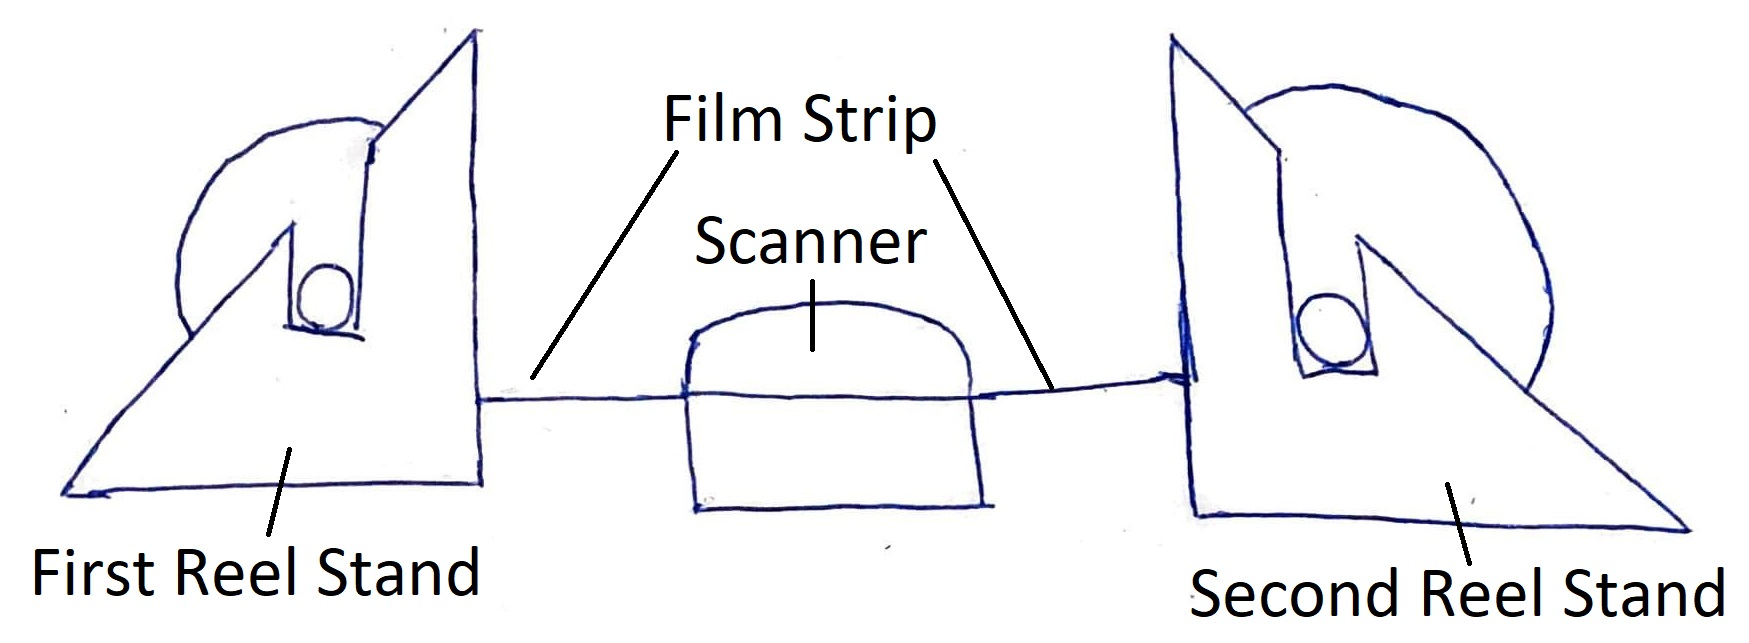
\includegraphics[width=0.7\linewidth]{Images/whole set up.jpg}
    \caption{A rough sketch of a hypothetical overall set-up including two reel stands and the scanner.}
    \label{fig: whole set up}
\end{figure}

Figures \ref{fig: reel stand side view} and \ref{fig: reel stand front view} show the side view and front view, respectively, of a hypothetical reel stand.
\begin{figure}[htb]
    \centering
    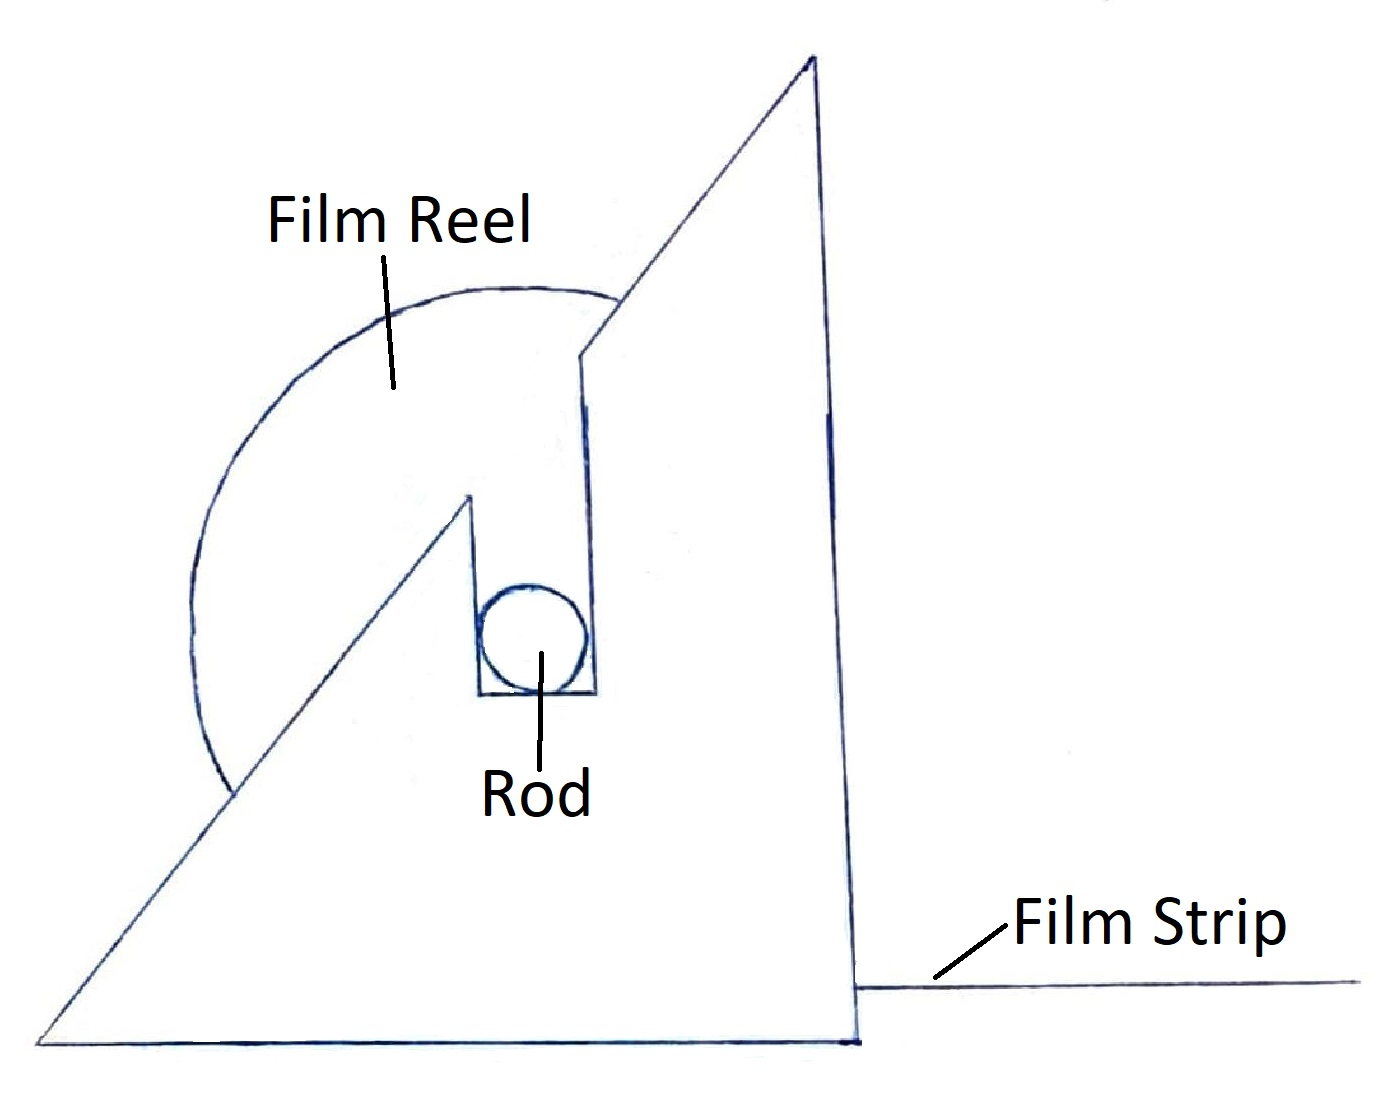
\includegraphics[width=0.5\linewidth]{Images/side view.jpg}
    \caption{A rough sketch of a hypothetical reel stand, from a side view.}
    \label{fig: reel stand side view}
\end{figure}
\begin{figure}[htb]
    \centering
    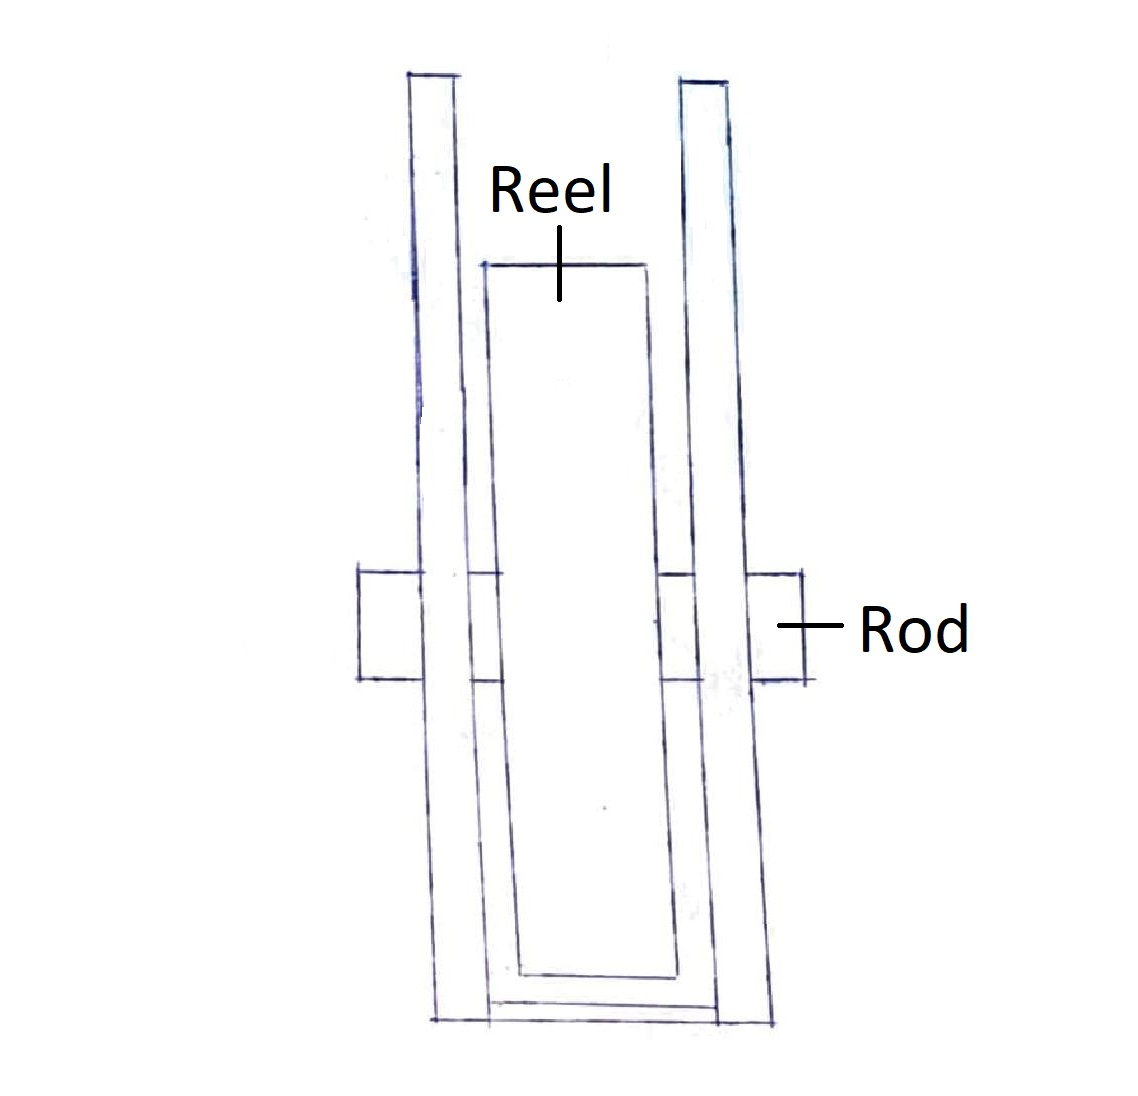
\includegraphics[width=0.5\linewidth]{Images/front view reel stand.jpg}
    \caption{A rough sketch of a hypothetical reel stand, from a front view.}
    \label{fig: reel stand front view}
\end{figure}

Construction of such reel stands should take 3-4 hours per stand, or 6-8 hours for both, using the same kinds of materials as the final design. The cost of the reel stand would be very similar to that of the final design, around \$80 total without scale or around \$50 total with scale.

The main reason our final design is superior to this triangular design is modularity. Our final design allows with different axle holes to be used with our stands, while this triangular design would demand one size of axle to fit the rod's slot. In our final design, we can simply use any size axle we like by drilling another whole in the wood sheets. We can also use screws as axles, while the triangular design may require wooden or metal rods to be machined such that they fit the rod slot and can firmly hold the reels. Finally, the triangular shape itself is mainly for aesthetics and reducing weight, which are not significant considerations for reel stands that are to be left in place in a science lab.

\subsection{Scanner: Previous Designs and Design Decisions} \label{scanneralts}
Perhaps the most significant component of this opportunity is the scanner used to digitize the film. In this section we explain the broad types of scanners and scanning services available, and the scanner type ultimately selected. There are two types of scanners for photography: flatbeds and feed. For movies or video there are also motion picture film scanners, which are more suited to work with film reels like ours. There are also scanning services offered by local businesses.

\subsubsection{Selected Alternative: Epson Perfection 4990 Photo} \label{selectedscannertype}
The scanner option selected for this project is the Epson Perfection 4990 Photo, a flatbed scanner. To meet Professor Bailey's desire to keep the film reel intact, we will use the scanner without a template, hence we do not need to cut the film nor do we risk any creasing of the film. Feed scanners either require the film to be cut, or are unable to scan shots of our size without significant modifications, so they are unsuitable. While motion picture film scanners do not require film to be cut and can likely scan our wide shots, they either have much too low DPI for our purposes or are too expensive to use. Finally, inquiries with local professional film-digital businesses have proven that they are unsuitable for our needs, unless we cut the film.

To justify the purchase of a new scanner, it had to meet our objectives and constraints on scan quality and have better scanning speed than the 4990. In tests we initially tested the 4990 to take about 6 minutes per scan at 4800 DPI for one of our shots, but we later reduced this to 4 minutes to 5 minutes.

Manufacturers of scanners always publish their scanners' DPI options, which helped us eliminate many scanners that did not meet the 4800 minimum. Interestingly, we encountered great difficulty in finding any official scanning speed measurements, as manufacturers either published results in confusing non-standard units (such as milliseconds per line, rather than the scan speed of a single transparency at a certain DPI) or did not publish any speed values at all. Thus, we had to rely on user reviews to measure scanning speed. 

Therefore, we consulted professional user reviews, often in the form of blogs, to obtain speed estimates. We tried to find a single blog with as many measurements as possible so the values would be consistent from scanner to scanner. Thankfully, a website, ScanDig, offered reviews of many scanners currently sold and previously sold \cite{ScanDig}. However, we again encountered problems. Many scanners that met our objectives and constraints are no longer sold. For example, the Canon CanoScan 9000F Mark II scanned a single standard $35 \ \text{mm}$ in 50 seconds at 4800 DPI \cite{canoscanspeed}. As one of our shots is about 3 times wider than a standard shot, the CanoScan should take about 2.5 minutes to scan one of our shots, about 2.5 minutes faster than what the 4990 can do. However, the CanoScan was discontinued in 2019. The Epson Perfection V800 Photo was also fast but discontinued \cite{v800scandig}. Other scanners like the Epson Perfection V600 Photo have reviews on ScanDig showing slowness compared to our 4990 for their older models, but their newer models have not yet been reviewed by ScanDig \cite{v600scandig}. Moreover, other online reviews do not give any quantifiable speed test for the such scanners.

The Canon CanoScan 9000F Mark II, for example, shows that significant scanning speed improvements over the 4990 are possible but may require a second hand scanner to be purchased. Ultimately, we decided not to pursue such options and instead use the 4990, due to the potential for an scanner being damaged in shipping, shipping too late for us to test it, or being faulty upon delivery due to previous use. The reel stands are compatible with any flatbed scanner, so purchasing a scanner can be done later if need be.

\subsubsection{Flatbed Scanners}
Flatbed scanners are like a household printer. To operate them you lift open the scanner’s hood, place your film in a  template (also called a holder or insert) if necessary, close the hood, and scan. These types of scanners allow one to scan a variety of types of film including slides, sections of reel, and large and medium format. The large scanning surface also allows many shots to be scanned at once. Moreover, most flatbed scanners automatically crop and cut scans when a template is used, potentially saving much editing time.

Some flatbeds run the risk of damaging many of our shots if we do not cut the film. Any length of film that will not fit in the template will be bent, and any length of film that does not fit under the hood will also be bent when the lid closes. Other flatbeds, like the Epson Perfection 4990 Photo selected, do not have this risk of damage because they do not require a template for the shots, hence the film can be placed flat on the mostly level surface. The film can then be advanced by unrolling more film from the reel and more scans can be taken.

\subsubsection{Feed Scanners}
Feed scanners operate by feeding in film into one end of the scanner and pulling it out the other end. Some feed scanners also have automatic ``batch” functions that will pull the film through automatically, to automatically scan a whole reel of film. To operate them you insert your film into on end of the scanner (some require templates, but not all). You then may need to line up your film’s first shot using a screen on the scanner. You then either begin automatically scanning and feeding, or you manually scan. If you manually scan, you need to pull the film out the other end of the scanner to line up the next shot and continue the process.

Feed scanners typically allow a much smaller variety of film than flatbed scanners, many only compatible with $35 \ \text{mm}$ film. The largest disadvantage of feed scanners is that they will only scan shots in standard sizes. We cannot use them with our shots because they are much too wide to be captured by the scanner. We also cannot easily split our shots into multiple sub-shots and digitally stitch them together because the scanner will leave small gaps between each sub-shot. Unless we hack the scanner in some way, or somehow over come the small gaps, we cannot use feed scanners.

\subsubsection{Motion Picture Reel Scanners}
Motion picture film scanners operate like automatic feed scanners, except with the advantage that they can take an entire reel without need to cut it. We had great difficulty finding good motion picture film scanners in any reasonable price range (\$40000 USD+). The primary limiting factor was the DPI of each frame, affordable motion picture scanners offered much less DPI than we need. However many businesses, including several around the University of Toronto, offer their services (see section \ref{localfilmbusinesses}).

The main disadvantage of motion picture film scanners will be that we will be returned a video by the scanner, which we need to separate into photos frame by frame in post editing.

\subsubsection{Local Film Businesses} \label{localfilmbusinesses}
One option for the scanning project was to offload the whole scanning and editing job to a local film-digital business. The obvious benefits to this are that we could avoid mistakes by having professionals complete the job, and we can focus our time instead on other portions of the HEP Capstone Project. However, because our film is on a reel, in a unique size, and we do not want to cut the reel, our scanning job introduces a lot of problems for local businesses. Many local businesses were able to scan each shot but would have to cut the reel to be able to do so.

We contacted a professional film photographer for advice, who suggested we contact Niagara Customs Lab. Niagara Customs Lab’s expertise is in scanning motion picture film (movie reels), so they are used to scanning without cutting a reel. We contacted Niagara Customs Lab and explained what we needed, but they explained that they did not have the exact equipment needed for such a task, and suggested we contact Frame Discreet.

We then contacted Frame Discreet, who said they were able to scan the reel under our conditions but would only be able to manage 72 DPI (since they would scan our film like video rather than photo), much lower than the 4800 DPI constraint. They also suggested that we might contact Downtown Camera, another local film service.

We contacted Downtown Camera who explained they would need to cut the reel. They also suggested that we contact Niagara Customs Lab. Clearly, we had exhausted all the professional options by this point without find one that was satisfactory to our needs.

%%%%%%%%%%%%%%%%%%%%%%%%%%%%%%%%% END SCANNING %%%%%%%%%%%%%%%%%%%%%%%%%%%%%%%%%%%


%%%%%%%%%%%%%%%%%%%%%%%%%%%%%%%%%%% MANUAL %%%%%%%%%%%%%%%%%%%%%%%%%%%%%%%%%%%%%%%
\newpage \section{HEP Experiment Manual}

\subsection{Detailed Description of Design Opportunity}\label{Design Opportunity_Manual}

The purpose of the HEP experiment is to analyze particle tracks to identify final state particles produced as the result of colliding particles in a bubble chamber. The experiment consists of using information about the incoming particle ($\pi^+$) and the interaction medium (super-heated liquid hydrogen) to measure the properties of the particles produced in resultant collision between the $\pi^+$ and the protons of the liquid hydrogen. The experiment analyzes digitized versions of the events as caught on film, which have been converted to high-resolution digital photos which can be viewed on a computer. Students use image tracking software to measure the momenta of particle tracks resulting from the collision. The two main events currently analyzed in the experiment focus on the identification of strange particles that are produced from the collision between a $\pi^+$ and a proton.
\newline

The previous version of the manual for the HEP experiment outlined the relevant physics involved in the bubble chamber particle collisions, as well as information about the experimental procedure. However, the engineering design team had been made aware of several issues with the manual, which necessitated a rewrite of the manual. The issues with the previous version of the manual can be summarized as follows:

\begin{itemize}
    \item The `Theory' section in the manual is too verbose, and fails to succinctly tie the experiment to modern high energy physics
    \item The current description of the 'Procedure' does not include any description of the current particle tracking software students use, 'Traxis'
    \item The manual often refers to old measurement procedures/equipment (e.g.: hand measurement of particle tracks) and physical parameters that are often not used in the actual experiment (e.g.: optical density, $dE/dx$ - ionization energy of a particle through the medium)
    \item Many aspects of the manual are found to be confusing for students and instructors, such as the $dE/dx$ information, and in such cases it is not clearly motivated why the information is necessary.
    \item The structure of the manual is overall not optimal for easy reading, and can be difficult to extract relevant information quickly.
\end{itemize}

The main issues with the manual were addressed by rewriting the outdated components (such as theory or procedure), while incorporating elements of the manual that are unambiguous in guiding students to performing the experiment. In other words, the manual was modernized to address the issues stated above.

\subsection{Final Design: Revised Manual}
The engineering design team has made several improvements to the HEP manual as were initially detailed in the Design Brief. We consider these improvements in three main sections of the manual, namely the \textit{Theory}, \textit{Experiment} and \textit{Appendix} sections. We consider these improvements in more detail in the following subsections. 

\subsubsection{Theory}\label{sec:updated_manual_theory}
The main issue with the theory section of the previous edition of the manual was that it was too verbose, and failed to succinctly tie the experiment to modern physics. From student and instructor experience, it was generally perceived to be confusing, and often slowed down students due to this. Hence, the main improvements to this section entailed conveying the relevant physics information to students while not tying them down in the details. This was achieved by making appropriate subsections within the theory section to address different topics in a manageable way. That is, the theory section was modularized to address different topics, while not being verbose. This change makes the manual more readable and also more accessible to students who have not seen the material before. New sections were also added as per the suggestion of Professors. The subsections within the theory section are as follows:

\begin{itemize}
    \item \textbf{Bubble Chamber:}
    This section deals with the discussion of the bubble chamber, an apparatus used historically to detect particles, which is the basis for the HEP experiment. It also discusses ionization energy and how to distinguish particle tracks in bubble chamber images. Finally, we provide a link to modern high energy physics. This section was slightly improved from the old manual.
    \item \textbf{Particle Physics:}
    This section seeks to succinctly explain the theory of modern particle physics at a level accessible to undergraduates. This is done by introducing the Standard Model of Particle Physics, which describes all the known fundamental constituents of the universe and their interactions. Then, conservation laws and their consequences are addressed. Finally, strange particle decays, which are of particular interest for this experiment, are addressed. This section was significantly improved from the old manual.
    \item \textbf{Relativistic Kinematics:}
    This section deals with the mathematical formalism used to analyze the bubble chamber photos in this experiment. It addresses the four-vector formalism, different frames of reference, and energy/momentum conservation. This is presented in a very brief manner, such that it is easily accessible and understandable to students referring to it to do calculations. This section was previously not present in the old manual.
\end{itemize}


\subsubsection{Experiment}\label{sec:updated_manual_experiment}
The main issue with this section in the previous manual was that the Procedure section did not include any useful descriptions of the particle tracking software Traxis. It was unfeasible to put the Traxis user manual within the procedure, however, so it was determined that it could be integrated as an appendix. This way, it could be referred to in the procedure without over-complicating it and being too verbose. The procedure was also changed to be more detailed with regards to how to use Traxis, such that students would be sufficiently guided without having the need to explicitly refer to the Traxis user manual. Cautionary statements were also added based on the experience of students and instructors regarding the technical issues faced when analyzing images in Traxis, mostly having to do with image down-conversion and the implications of this on momentum measurements. The order of the procedure was also improved, and any unnecessary references to old equipment or procedures were removed and/or updated. Overall, the steps were made much more clear such that they are easier to follow. Improvements were also made to the Further Studies subsection, where some guidance was added for one of the additional steps. 

\subsubsection{Appendices}\label{sec:updated_manual_appendices}
The previous appendices made reference to outdated measurement procedures, and did not otherwise any other information that may be useful to the experimenter. The appendices were vastly improved, with new sections being added to improve the experimenter's experience. The entire Traxis user manual was added as an appendix, making it easier for the experimenter to access the user manual in one place. This was also updated to reflect changes that were made to the software. In the future, any new changed to Traxis can be conveniently recorded within the manual itself. Additionally, information about the natural unit system often used in HEP, as well as information about the Particle Data Group (PDG), which is an online compendium of the latest findings in (mostly) experimental HEP, were added. Lastly, supplemental information relating to the stopping power and range of protons in hydrogen was also added for interested students.

\subsection{Objectives, Metrics, and Our Design’s Performance  }
In the following section we consider the objectives and metrics that guided our design process of the HEP manual. Note that metrics discussed in this section are qualitative in nature, and hence should be seen as general guiding principles rather than exact measures. Here, we partition the objectives into various sub-objectives, indexed as components of the manual; these components must satisfy various requirements in order for them to be satisfactory. We also indicate the performance of the revised HEP manual in satisfying these metrics.

\subsubsection{DFX Considerations}
Several key aspects of a manual facilitate the ability to perform a good experiment - thorough, guided details, and concise yet informative descriptions of information pertaining to the experiment. In this, we identify that we must design for readability. Additionally, from our discussion of the manual in section \ref{Design Opportunity_Manual}, we can identify that it is necessary to modernize the manual to accurately reflect the state of modern high energy physics. Additionally, this and other information presented in the manual must be conveyed at a level appropriate for an undergraduate student to understand, and must provide just the exact amount of details necessary to complete the experiment, while providing a flavour of advanced topics for future study. Hence, we must also design for practicality and modernity.

\subsubsection{Introduction \& Theory}
The introduction and theory sections must provide a good background of the physics involved in this experiment. In particular, it must cover the relativistic kinematics as well as the conservation laws used in the calculations in the experiment. In addition to this, it must also provide a historical background to the physics being explored, and tie this to modern experiments (e.g. at CERN). It must convey these points without being verbose, so as to not distract the student from the experiment at hand. 

\paragraph{Metrics}
\begin{itemize}
    \item Description: Provide a good historical and physics background to enable the student to thoroughly understand the experiment at hand.
    \item Measurement: Feedback from users of the manual, such as students, TAs, and Professors.
    \item Final Performance: See section \ref{sec:updated_manual_theory} for information regarding the changes made to this section. Professor Bailey has indicated that the introduction and theory sections are satisfactory. This metric adequately satisfied the engineering design team and our stakeholders’ desires for improved introduction and theory sections.
\end{itemize}

\subsubsection{Pre-Experiment}
In order for the student to become familiar with the software and method of analysis, they must perform preliminary exercises. These will allow the student to identify several different types of events and decays that can be seen in the digitized film roll events (bubble chamber collisions). This section was very verbose and at times confusing in the previous version of the manual. Hence, it is imperative to make this section concise and coherent. It is also important to introduce the student to the particle tracking software, Traxis. Students must become accustomed to its use and know how to properly use it before analyzing either of the main events. Thus, it is a good idea to integrate elements of the Traxis manual into this section.

\paragraph{Metrics}
\begin{itemize}
    \item Description: Familiarize students with various types of events (decays, spirals, secondary interactions) that can be seen in the bubble chamber events. Thoroughly explain Traxis and its use, perhaps through examples as well as concise descriptions from the manual.
    \item Measurement: Feedback from users of the manual, such as students, TAs, and Professors.
    \item Final Performance: Instead of integrating Traxis into this section, it was decided that it would be better to include it into the appendix section. See section \ref{sec:updated_manual_experiment} for additional information regarding the changes made to this section. Professor Bailey has indicated that the pre-experiment section is satisfactory. This metric adequately satisfied the engineering design team and our stakeholders’ desires for an improved pre-experiment section.
\end{itemize}

\subsubsection{Experimental Procedure}
The procedure in the previous manual is slightly outdated in the fact that it makes reference at times to experimental steps that are confusing (e.g. $dE/dx$ measurements). In consultation with Professors who have supervised the experiment, it has been mentioned that several such aspects often end up confusing the student rather than helping them get through the experiment (see section \ref{Stakeholders_manual_TA/Prof}). Hence, it is important to omit confusing elements of the procedure while strengthening parts which are not explained very well.

\paragraph{Metrics}
\begin{itemize}
    \item Description: Make the experimental procedure concise and unambiguous to the student.
    \item Measurement: Feedback from users of the manual, such as students, TAs, and Professors.
    \item Final Performance: The experimental procedure was changed to be more systematic, removing unnecessary references and overall trimming down the procedure to the bare minimum. References to Traxis were also included. See section \ref{sec:updated_manual_experiment} for information regarding the changes made to this section. Professor Bailey has indicated that the experimental procedure section is satisfactory. This metric adequately satisfied the engineering design team and our stakeholders’ desires for an improved experimental procedure section.
    
\end{itemize}

\subsubsection{Miscellaneous}
It is important to consider that the manual must also incorporate any changes/additions made to the software, as well as thorough descriptions of software used currently (e.g. Traxis). One obvious way to achieve this is to merge the Traxis documentation with the HEP manual, perhaps in the form of an appendix. It is also important to keep elements of the old manual which mention how hand-measurements are made on the bubble chamber images to measure momentum, as these concepts form the basis for what Traxis automates, and is thus good to include for student understanding. It is also worth considering the possibility of adding the $dE/dx$ tables/graphs mentioned in section \ref{Stakeholders_manual_TA/Prof} to aid the student in understanding these parameters. 

\paragraph{Metrics}
\begin{itemize}
    \item Description: Integrate information about software used in the experiment. Include miscellaneous information in a coherent fashion so as to improve the understanding of the user of the manual.
    \item Measurement: Feedback from users of the manual, such as students, TAs, and Professors.
    \item Final Performance: General improvements as well as stylistic changes to the manual were made to improve readability and accessibility for experimenters. In particular, see sections \ref{sec:updated_manual_theory} and \ref{sec:updated_manual_appendices} for additions to the theory and appendix sections of the manual, respectively. In particular, changes to Traxis were recorded in the manual, and the Traxis user manual was integrated with the HEP manual for ease of access. Professor Bailey has indicated that the overall HEP manual is satisfactory. This metric adequately satisfied the engineering design team and our stakeholders’ desires for integrating information about Traxis into the manual.
\end{itemize}

\subsection{Stakeholders}
Here we analyze the primary stakeholders for the HEP Experiment Manual.

\subsubsection{Professor David Bailey}
Professor Bailey is the head instructor of the advanced physics lab, and has thus contributed greatly to the development of the HEP experiment. Professor Bailey's preferences for the manual were key in making design decisions with respect to how we chose to write it. In particular, Professor Bailey had outlined several key aspects of the manual that he wanted addressed for the new version, which are listed in Section \ref{Design Opportunity_Manual}. Over the course of our consultation process with Professor Bailey thus far, we have had several discussions with regards to how the manual should be modernized and compacted to make it more accessible to students and instructors. Through this process, we were able to get significant guidance with respect to the structuring and content of the manual. Through periodic checks by Professor Bailey, the manual was iterated upon to maximize its effectiveness.

\subsubsection{HEP Students}
The HEP students are a critical stakeholder in the development of the manual. Their understanding of the physics involved and experimentation process is key to the success of the revised manual. The past version of the manual has been described as confusing due to the long section on theory and brief description of the experimental procedure, which is confusing to students. There are several sections which are outdated, and were thus updated to reflect advances in modern physics. Both authors of this report were previous HEP lab students, so we have experienced these issues firsthand. Addressing these issues was the first priority in updating the manual. From this perspective, we were able to minimize confusion with regards to the manual, and make the sections as unambiguous and clear as possible. 

Though direct consultation with students was not possible due to the circumstances, we were able to systematically eliminate many ambiguities of the previous manual through an iterative process of checking. Although the engineering design team had initially planned to receive feedback from actual HEP students regarding the manual, no feedback was received from any students. We assume this was due to conflicting schedules; we managed to mitigate this lack of feedback by designing the manual from the perspective of an HEP student to improve readability and accessibility. We were assisted by the fact that both members of the engineering design team were previous HEP students.

\subsubsection{Professors/TAs}\label{Stakeholders_manual_TA/Prof}
Professors and TAs in the Advanced Physics Lab experiments play an integral role in the experience of the students who perform the experiments. It is thus imperative that both of these stakeholders thoroughly understand and can follow along easily with the manual. Any ambiguities in the manual make it a hindrance for the Professor and TA to guide the students; additionally, any key omissions of information also make it difficult for them to explain concepts critical to the success of the experiment. Hence, in consulting with these stakeholders, it was important to ensure that they agree with the changes to the manual to optimize teaching of students. The engineering design team has been in frequent contact with Professors who supervise the HEP experiment in a continuing process of consultation to improve various aspects of the manual. Some of the suggestions provided can be summarized as follows:

\begin{itemize}
    \item Make clear what energy scales are meant by ``high-energy".
    \item References to the Particle Data Group (PDG) \cite{PDG}.
    \item Clarify the meaning of the $dE/dx$ values by collecting them in a table/Python script.
    \item Streamline the theory portion of the manual to make it more concise.
    \item Reference the CERN, SLAC experiments.
    \item Mention issues with image quality down-conversion resulting in skewed momentum measurements.
\end{itemize}

We were able to implement many of these changes into the revised manual. The first point was omitted however, as advised by Professor Bailey. 
%%%%%%%%%%%%%%%%%%%%%%%%%%%%%%%%% END MANUAL %%%%%%%%%%%%%%%%%%%%%%%%%%%%%%%%%%%%%


%%%%%%%%%%%%%%%%%%%%%%%%%%%%%%%%%%% SOFTWARE %%%%%%%%%%%%%%%%%%%%%%%%%%%%%%%%%%%%%
\newpage \section{Software}
\subsection{Detailed Description of Design Opportunity}\label{Detailed Description_Software}
The engineering design team had been made aware of additional improvements that could be made to the software currently in use in the HEP experiment. Currently, students use image tracking software to measure the momenta of particle tracks in various collision events. This software, Traxis, is capable of measuring the momenta of particles, the angle between particle tracks, as well as the optical density of tracks. The optical density parameter could in principle be related to the ionization energy of a particle through some medium, $dE/dx$. %problematic last sentence

In our discussions with Professor Bailey, he had mentioned that he would like for there to be improvements to the image tracking software. While there were many potential features that could have been added, the design team decided to frame the improvements around ``quality of life" features for the user, thereby reducing our scope to match our time-frame. Thus, the improvement of focus was to implement some method to intuitively or easily recall previously saved analysis sessions such that multiple sessions could be recalled easily and compared or modified. By implementing such a method, students could recall previous sessions and modify them to iteratively improve their results and reproduce them, two important aspects of all physics research that were notably difficult to perform in the previous version of Traxis.

\subsection{Final Design: Updated Traxis Software}
Changes to Traxis were made to implement the proposed analysis recall feature with a window to show saved sessions (JSON files) in a selected folder and a button to select the session folder. The window is shown in figure \ref{fig:traxis_gui} as the ``Saved Sessions" folder, while the ``Load Folder" button promptly opens a file browser to select a folder. Figure \ref{fig:traxis_gui_filled} shows the ``Saved Sessions" window with several sessions available.
\begin{figure}[htb]
    \centering
    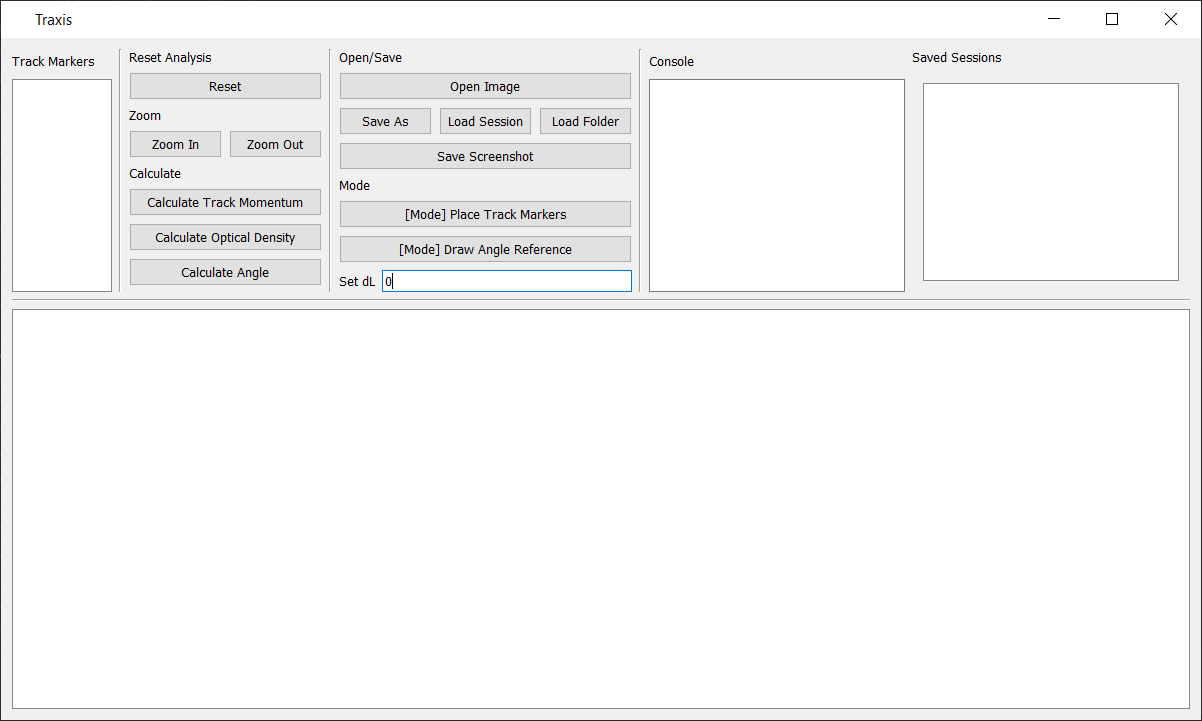
\includegraphics[width = \linewidth, height = 12cm]{Traxis_photo.png}
    \caption{The Traxis GUI on startup}
    \label{fig:traxis_gui}
\end{figure}
\begin{figure}[htb]
    \centering
    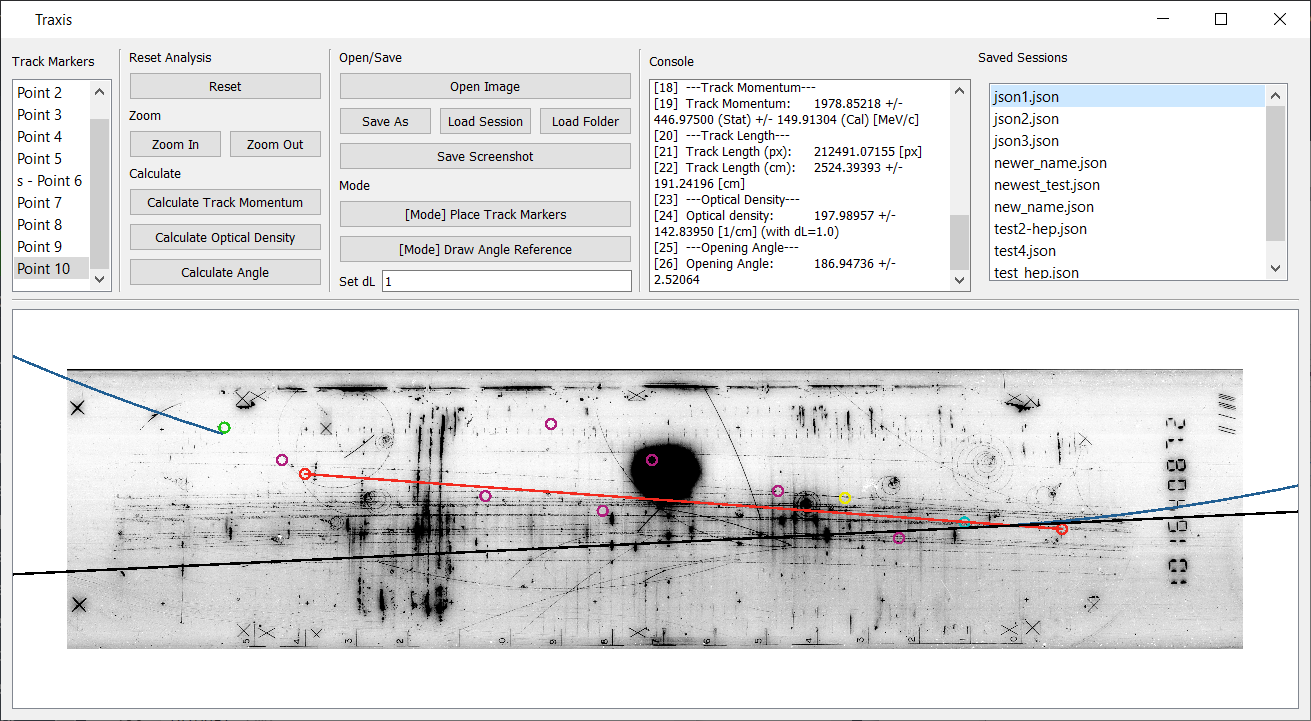
\includegraphics[width = \linewidth, height = 12cm]{traxis_filled_photo.PNG}
    \caption{A filled Traxis GUI with many saved sessions in the window. The console shows computed track momentum, reference angle, optical density, and other fit parameters. The image viewer window below shows track markers (circles), along with the reference line (red line), fitted track (blue line), and tangent to the fitted track at the reference line point (black).}
    \label{fig:traxis_gui_filled}
\end{figure}

The ``Saved Sessions'' window shows all the saved sessions in the currently selected folder. A folder can be selected using the ``Load Folder" button, or by using the ``Load Session" button. If the ``Load Session" button is used the selected session's folder will be automatically selected to be shown, and the selected session will be loaded into Traxis. All the sessions located in the session's folder will also be loaded into the ``Saved Sessions'' window. If the the ``Load Folder" button is used, a folder can be loaded into the window without immediately loading a session into Traxis. Automatically changing the selected folder when ``Load Session" is used was implemented as a ``quality of life" feature, to reduce the user's need to manually change the folder after they have already selected a session.

Sessions in the ``Saved Sessions" window can be double clicked to load them into Traxis. This is another significant ``quality of life" feature that was not present in the previous version of Traxis. Users no longer need to use the file browser to navigate to a folder with saved sessions each time they want to load a session, instead they can simply use Traxis' GUI. Moreover, quickly loading sessions allows users the ability to iterate sessions by modifying them and saving them quickly, with the ``Saved Sessions" window being updated each time a new session is saved to it. In this way, users quickly see previous versions of their analysis.

The ``Load Folder" button opens a file browser window through which users can use their computer's native file browser to select a folder to load in the ``Saved Sessions" window. This feature was designed to be as simple as possible as much of the workflow and ``quality of life" features are implemented in the ``Saved Sessions" window itself. The ``Load Folder" button also gives the user a method to see the files in a folder without clearing their current session because the ``Load Session" button will load the selected session along with updating the ``Saved Sessions" window, hence clearing whatever the current session was. This is another ``quality of life" feature because users can now, for example, load a folder to remind themselves of the file naming scheme they are using in that folder without having to clear their session.

Notably, there is a ``Save As" button to save the session to a new file, but there is no ``Save" button. We chose not to implement a generic save feature (one that simply saves over the current session's file name) because we wanted to encourage the user to document each iteration of their analysis in new files. Moreover, a useful ``Save" feature should quickly save over the current file, without asking for confirmation (if it asked for confirmation it might as well just be a ``Save As" function), however in the case of HEP analysis it is very dangerous to save an analysis without confirmation because changes and previous versions are very difficult to track (or cleared entirely once the file is saved), hence greatly limiting reproducibility. Thus, we ultimately decided not to implement a ``Save" button at all.

For comparison, the previous version of Traxis did not have the same functionality as described above. As can be seen in figure \ref{fig:old_traxis}, a few additional buttons and the Saved Sessions window were added to the GUI. In particular, the ``Save'' button was changed to ``Save As'' to properly reflect its function (that is, it saves a new file, which the user has to specify the name and location of in the file dialog which is opened by Traxis). The ``Load'' button was split into a two load buttons, as were described above.

\begin{figure}[htb]
    \centering
    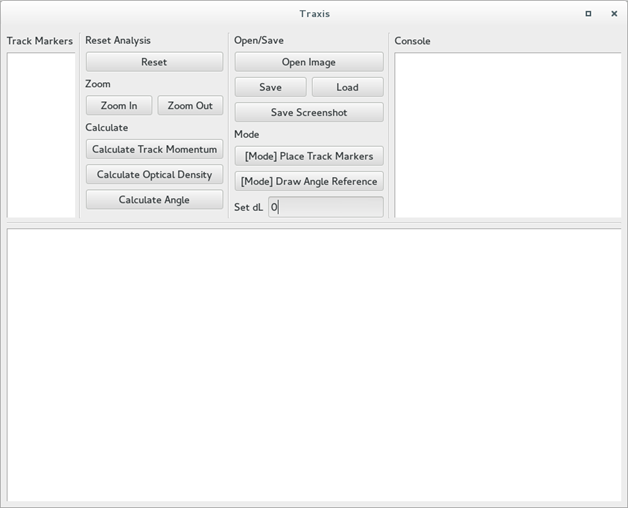
\includegraphics[width = \linewidth, height = 12cm]{old_traxis.png}
    \caption{The previous version of the Traxis GUI}
    \label{fig:old_traxis}
\end{figure}

\subsection{Objectives and Metrics}
Note that metrics discussed in this section are qualitative in nature, and hence should be seen as general guiding principles rather than exact measures. Most of the metrics were validated by extensive user testing of the software (such as within the GUI).

\subsubsection{DFX Considerations} \label{dfx software}
Many of the design decisions for the software component of this project arose from the student experimenters' use of the software; therefore, we mostly designed for usability. In this design opportunity, we define usability as the level to which the software is easy to use and understand. Usability informed much of software's interface design. In the end, we observe that the software was fairly intuitive to use, hence it was usable. The software was also properly documented both in the code as well as in the HEP manual, so both users of the software and those wishing to make changes to the code will find that both elements are rather accessible.

In designing the software, speed was also a consideration that was made, however extensive testing of the software indicated that this was not an issue. For instance, opening the sessions via the ``Saved Sessions'' window took as long if not less time than as they did previously  while using the ``Load'' button. Absolute speed varies by computer, but this general observation was observed to hold true.

\subsubsection{Usability/Accessibility of Software}
As mentioned in section \ref{dfx software}, the software must be usable to the experimenter. The software must be developed such that first-time users can understand it without extensive support of the TAs (demonstrators) or professors (supervisors).

\paragraph{Metric: Simplicity of Use}
\begin{itemize}
    \item Description: The software, as analyzed by students and demonstrators who use the software, must find it satisfactory to use, and simple enough so that one can use the software without having to extensively refer to the manual, professors, or TAs. 
    \item Measurement: Qualitative feedback received from users, perhaps in the form of a numerical user survey.
    \item Final performance: The final design is very simple to use. Only two more components were added to the GUI, and they can be interacted with using the user's computer's native file browser or simply double-clicking with a mouse. Moreover, unambiguous button names and window names simplify the experience. 
\end{itemize}

\subsubsection{Speed of Software}
As the student experimenters have limited time to complete the experiment and typically makes tens to hundreds of measurements for multiple particles, the software features' speeds must not impede the experiment's completion.

\paragraph{Metric: Feature Speed}
\begin{itemize}
    \item Description: This metric measures the time taken by the software to produce the result of a feature, on average, lower is better.
    \item Measurement: Milliseconds; begin measuring when feature is executed, end measuring when result is returned (may have to use programming tools to measure).
    \item Final performance: The added features are as fast as the previous version of Traxis. Loading a folder of multiple sessions takes as long as loading a single session, and loading a session from the ``Saved Sessions" window is as fast as using the ``Load Session" button, or loading sessions in the previous version of Traxis using the ``Load'' button.
\end{itemize}

\subsection{Stakeholders}
This section analyzes each stakeholder in relation to the software design opportunity, the preferences they expressed, how we addressed these preferences, and our interactions with them. We also outline how their preferences guided our design decisions along the way.

\subsubsection{Professor David Bailey} \label{dbaileysoftware}
Professor Bailey is the foremost stakeholder for this design opportunity. He is the coordinator of the Advanced Lab, and thus is closely tied to the pedagogy of the HEP experiment. Professor Bailey will have final control over which features will be released to students, by deciding whether they are supportive of the student experimenters' learning.

Professor Bailey had expressed several preferences that inform our design decisions and objectives. Firstly, Professor Bailey had outlined several extensions to the software he would like us to make. These include methods to calculate total and differential cross sections and hadronic resonances. As explained in section \ref{sec:previous_design_considerations}, these features could not be implemented without significantly changing Traxis. Secondly, he expressed interest in allowing the software to still allow mistakes to be made by students, as this would positively impact their learning experience. For instance, the errors encountered could be systematic, and thus could be addressed in their experimental process as such. To address this preference, we did not modify the computational features of the software, so students can still make the same errors they previously could. However, our features make the over workflow of Traxis easier, hence when students do make mistakes they can easily iterate their erroneous analysis to correct it. 

Our changes to Traxis were not as extensive as the list of items provided by Professor Bailey due to time constraints. However, the engineering design team believes that the changes made to the software will have a measurable impact on the HEP student experimenters' experience. 

We have had very regular contact with Professor Bailey, including several emails a week and a weekly 30-60 minute meeting.

\subsubsection{HEP Student Experimenters}
HEP student experimenters are important stakeholders because they will be the main users of the software.

Both members of the engineering design team were HEP student experimenters in the past, so we have used our own experiences as a proxy for the experience of HEP students in the lab. Moreover, Professor Bailey in his experience as the Advance Lab coordinator has interacted with many HEP student experimenters, so he has helped support our proxy. There are various ``quality of life" preferences student experimenters have, including: automatic uncertainty calculations, descriptive error messages, and automatic unit conversion. However, many of these preferences may have to be rejected in favor of Professor Bailey's preference to allow students to make mistakes with the software to support their learning (see section \ref{dbaileysoftware}). However, the features implemented allow students to more easily use the software and have an overall more enjoyable experience. Most importantly, students can now very easily iterate over their previous analysis so any errors they previously made can be corrected once they learn how and why they made an error.

Regular internal discussion between the designers and meetings with Professor Bailey have been a proxy for interaction with HEP student experimenters. Due to negligible interaction with any current HEP experimenters, the engineering design team's experience was used as a proxy; our design decisions were thus impacted by our extensive testing protocol.

\subsubsection{Scan Operators} \label{scanopps software}
Scan operators are the people who will be scanning the film strips that produce the photos that are used in the HEP experiment (see section \ref{scanopsscanning}).

The main preference of the scan operators is to have a short overall scanning process, which is partially dependent on the minimum DPI (effectively image quality) needed for each scan; higher DPI means longer scanning time per scan. The minimum DPI of each scan is largely dependent on the software features implemented as the software may require higher DPI for better results, or even to work at all. Thus, the preference of the scan operators in regards to the software can be interpreted as wanting software features to work with only the ``minimum" DPI. The software works with different image DPI; in particular, there is no specific threshold for DPI that the software enforces. Hence, the scan operators have freedom in choosing the optimal settings as constrained by their scanning equipment. However, as explained in the Film Scanning opportunity, the minimum of 4800 DPI was selected, so the scan operators ultimately had no choice in what DPI to use.  

\subsubsection{Other Stakeholders}
Other stakeholders for this design opportunity include the supervising professors for the HEP experiment and the Advanced Lab teaching assistants who act as supporting demonstrators. The preferences of these stakeholders are met by the preferences of Professor Bailey and the student experimenters' preferences, so separate analysis is not needed.

\subsection{Previous Design Considerations}\label{sec:previous_design_considerations}
In this section we elaborate on the design decisions made that led to certain features not being implemented in the final version of Traxis.

\subsubsection{Ionization Density} \label{section: ionizationenergy}
In our discussions with Professor Bailey, we had initially thought to include a feature in Traxis whereby we would map some sort of an analytical correspondence between the ionization density (as discussed in the HEP manual; a theory parameter) and the optical density (available from Traxis; an experimental parameter). This would allow for more accurate identification of particles based on the optical density of their tracks. However, some experimentation with bubble chamber images in Traxis showed that the spread of optical density and momentum of pion tracks has a significant variance, hence complicating any attempt at analytically connecting the two parameters (see figures \ref{fig:momentum_distribution}, \ref{fig:ionization_distribution}). Further discussions with Professor Bailey revealed the physics complexities of the problem; that is, it was not clear exactly how this analytical correspondence would be established in theory. For these reasons, this feature was not implemented.

\begin{figure}
\centering
\begin{minipage}{.5\textwidth}
  \centering
  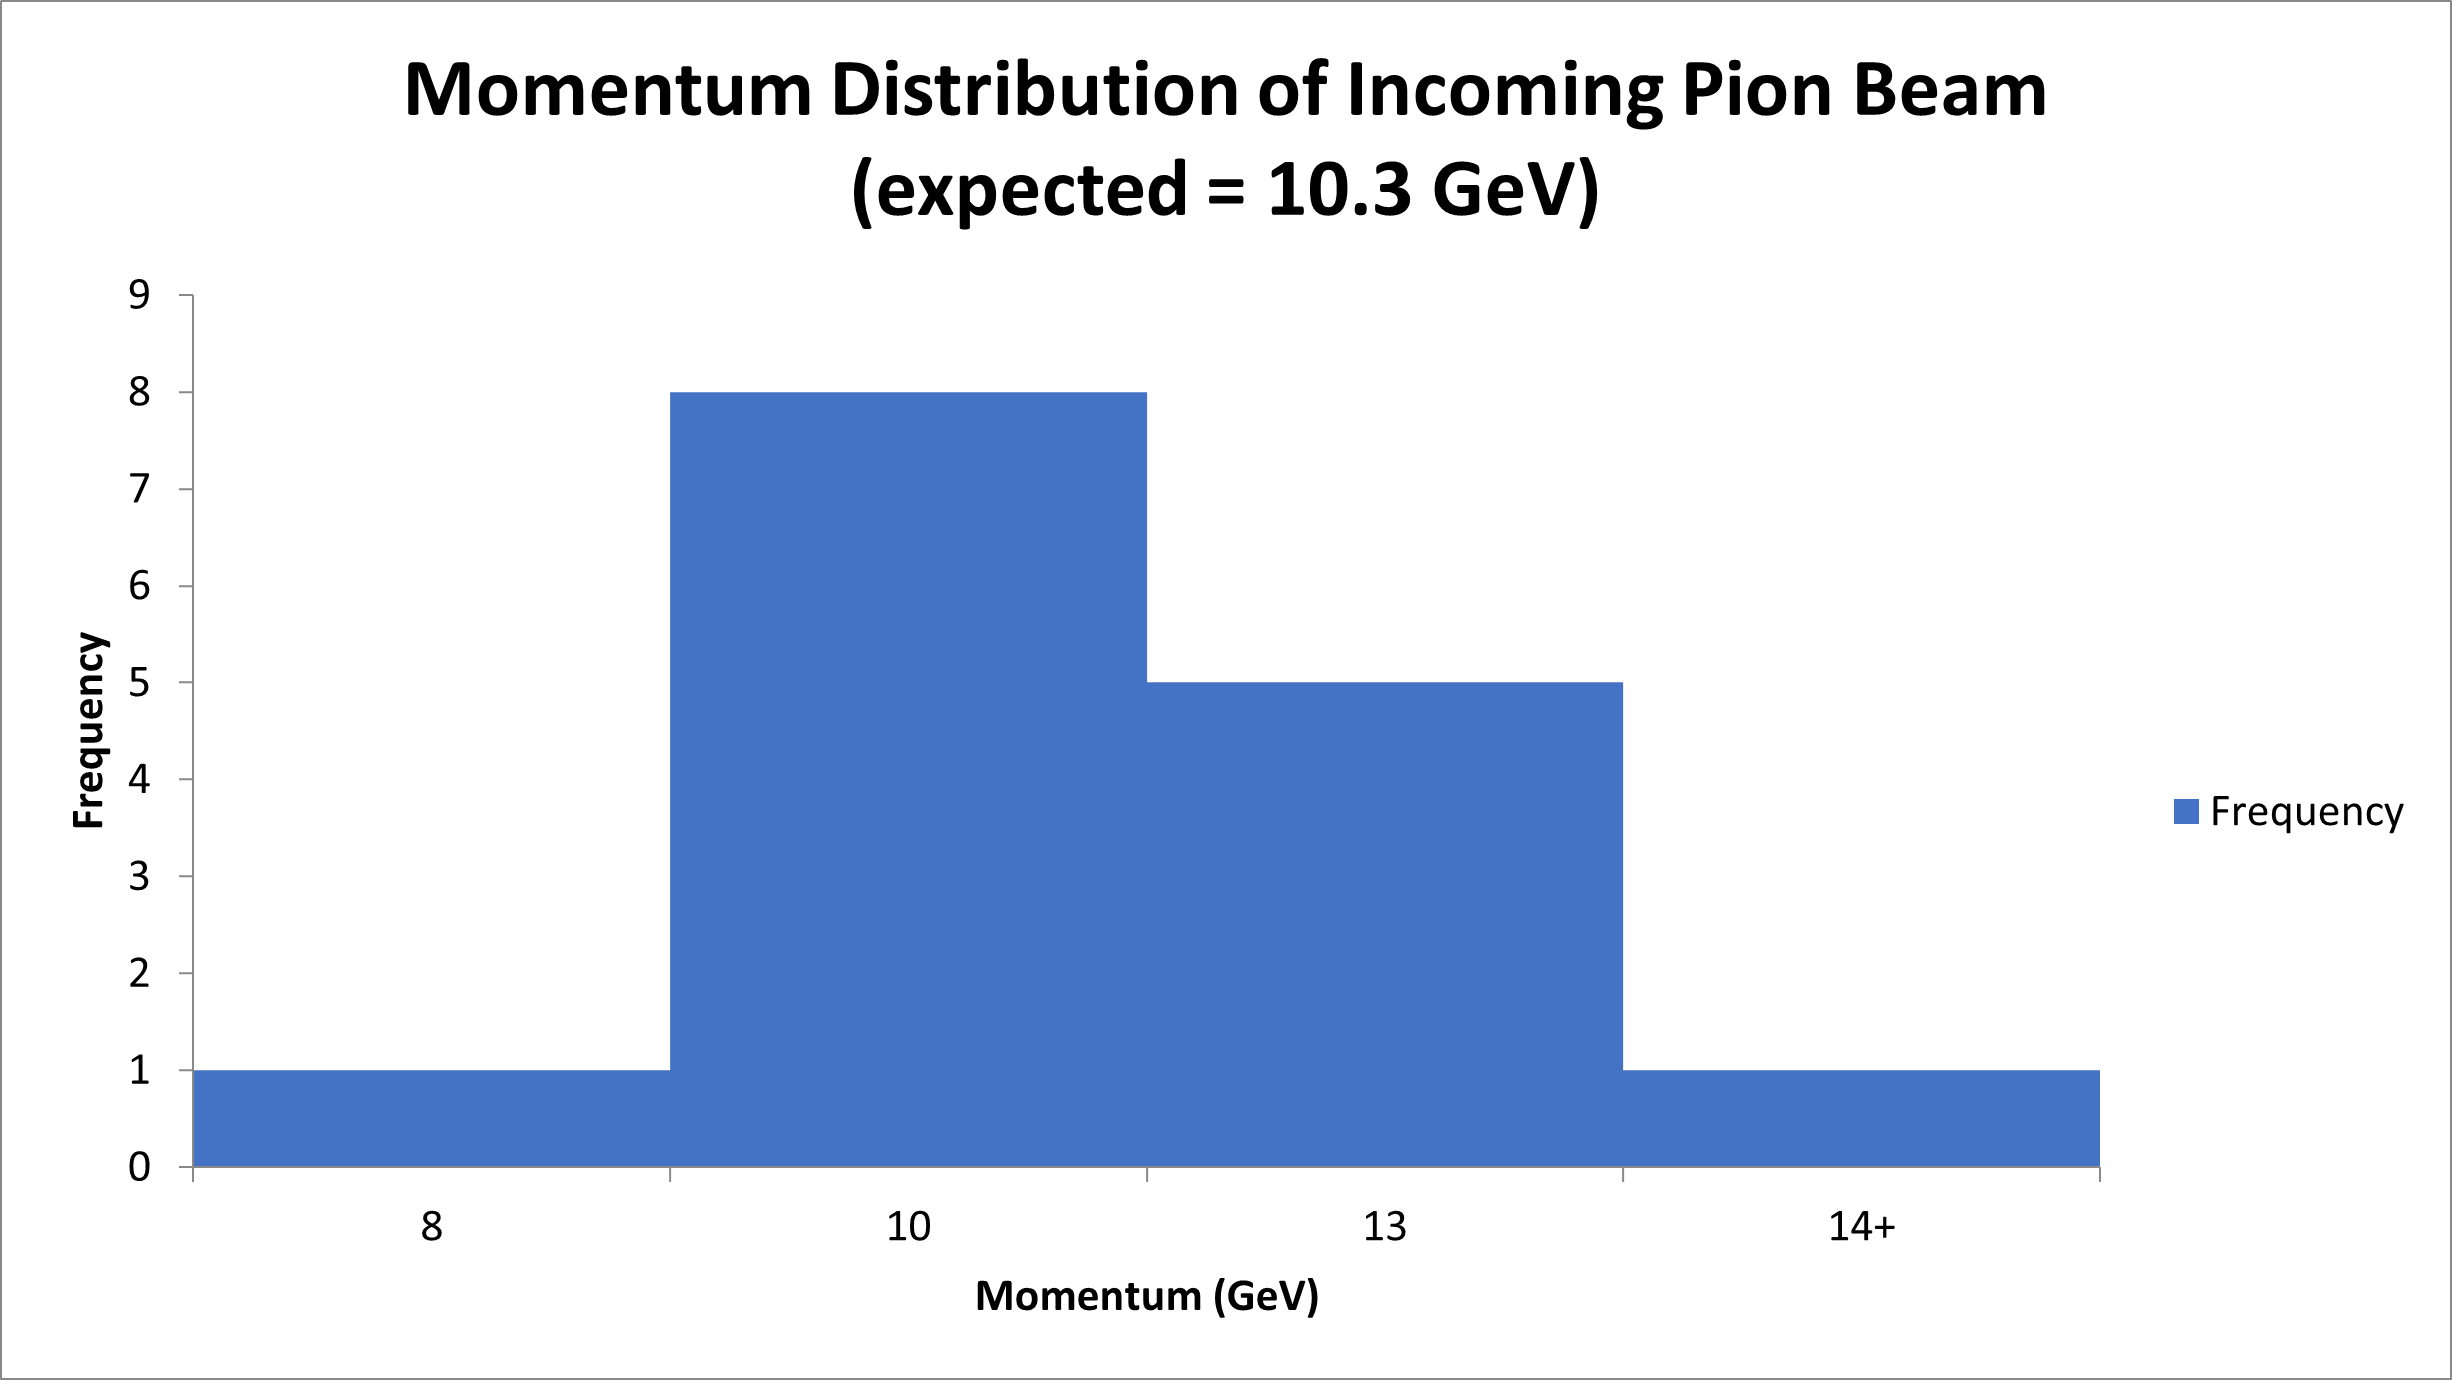
\includegraphics[width=\linewidth, height = 6cm]{momentum_distribution.png}
  \captionof{figure}{} %Momentum distribution of incoming pion beam.
  \label{fig:momentum_distribution}
\end{minipage}%
\begin{minipage}{.5\textwidth}
  \centering
  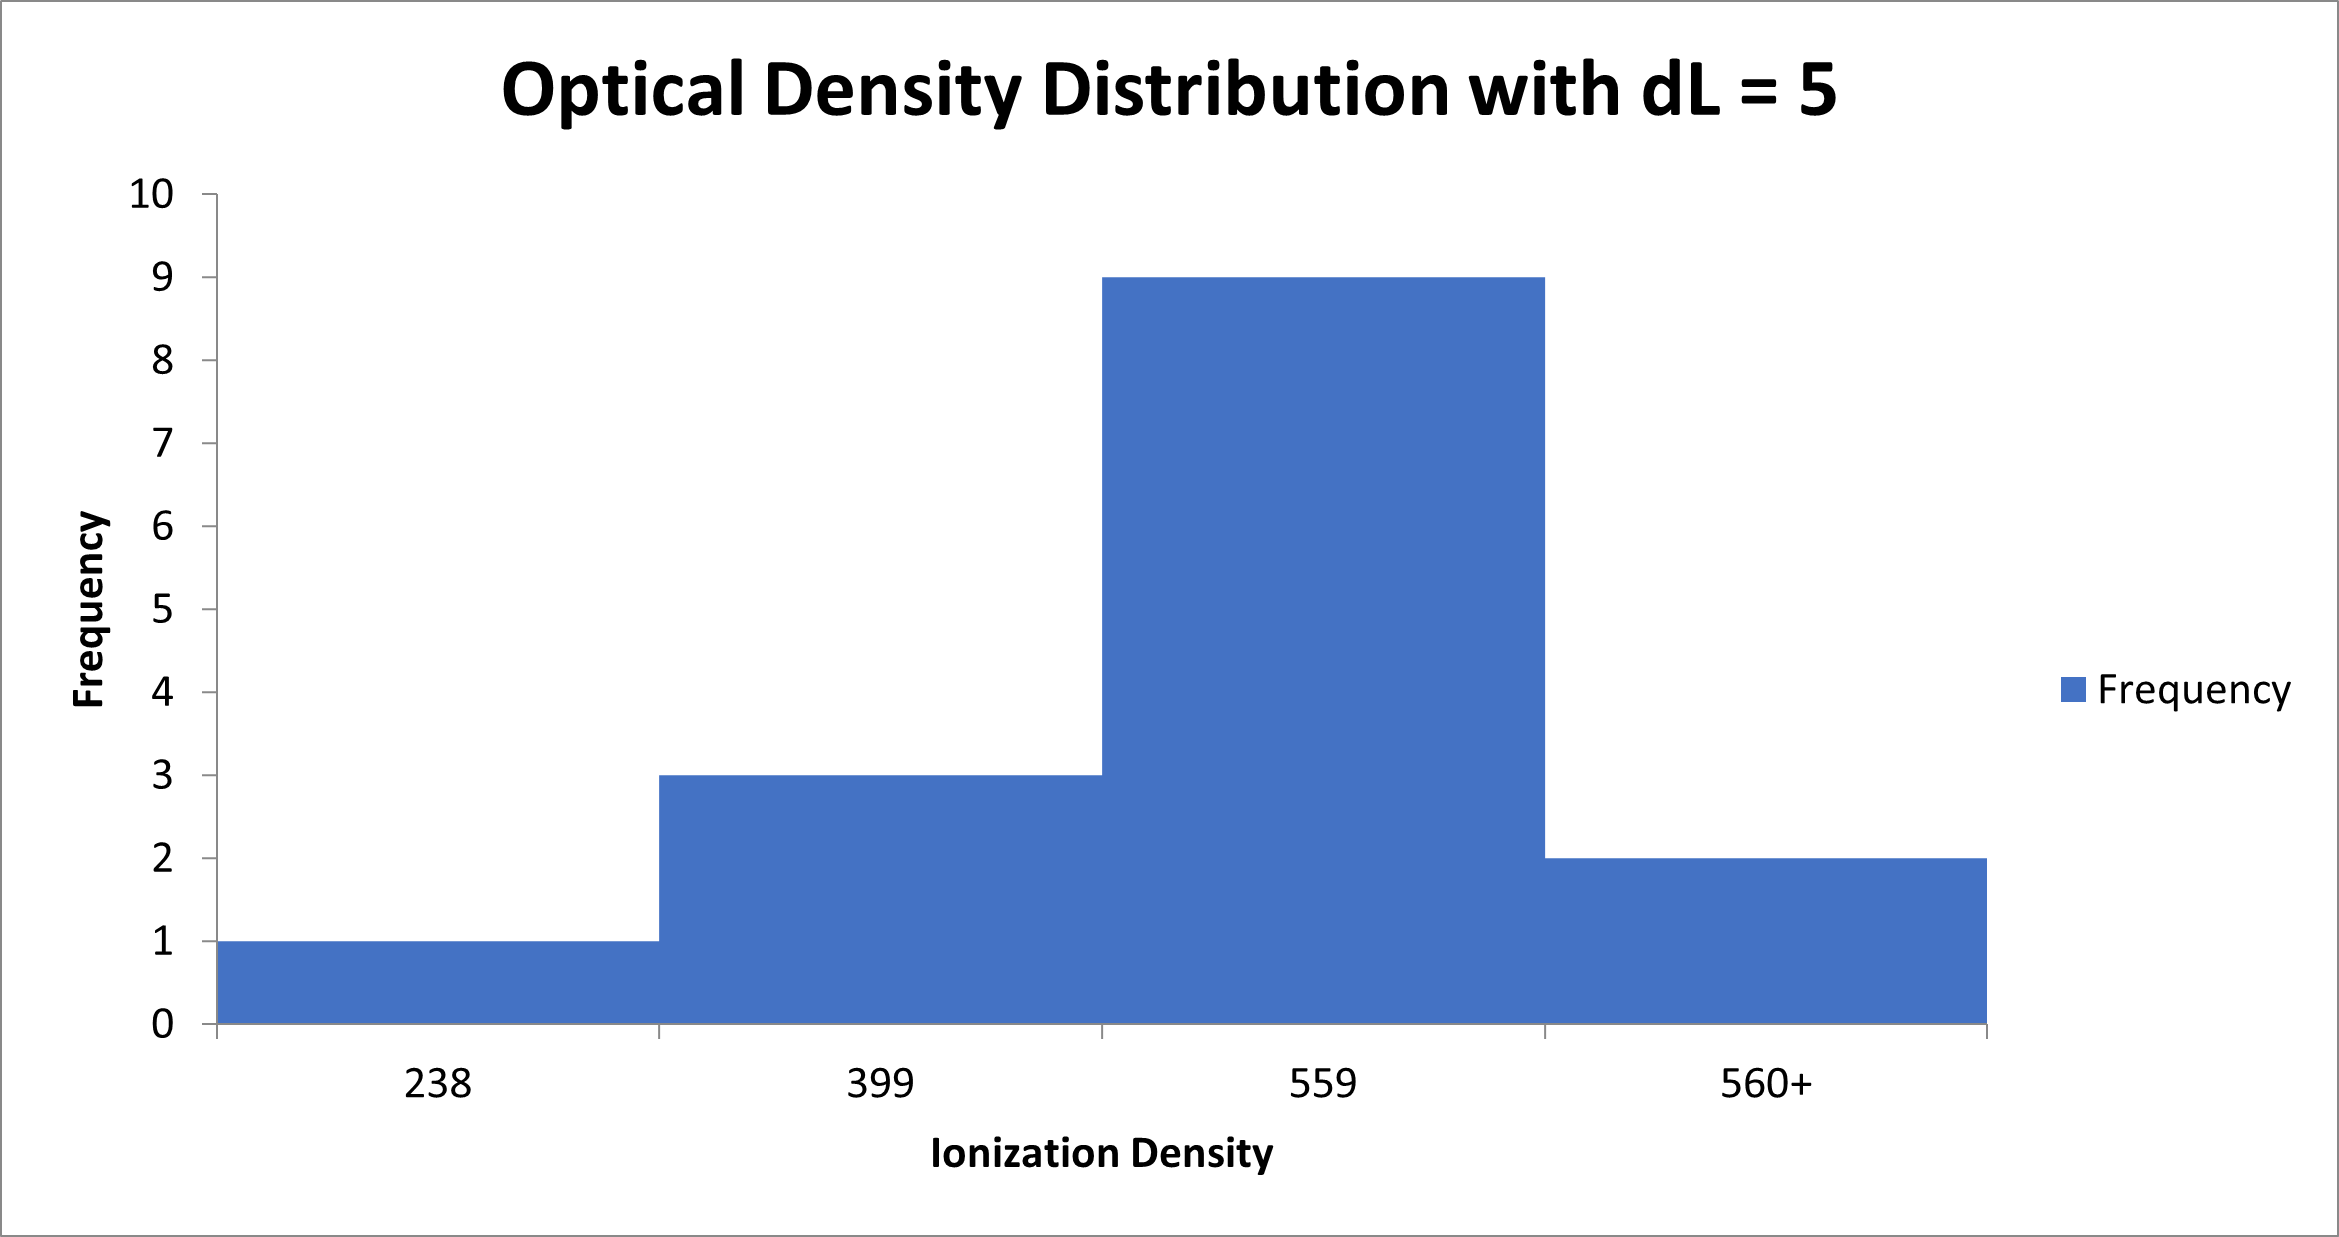
\includegraphics[width=\linewidth, height = 6cm]{ionization_distribution.png}
  \captionof{figure}{}%Optical density distribution of incoming pion beam.
  \label{fig:ionization_distribution}
\end{minipage}
\caption*{\textbf{Figures 15, 16:} Figure 15 is the momentum distribution of incoming pion beam, while figure 16 is the optical density distribution of incoming pion beam. Measurements made in Traxis using different bubble chamber images yielded the distributions of momentum and optical density above. These distributions indicate that the spread of momentum and optical density for a consistent set of measurements makes it hard to analytically connect to the ionization density due to the observed variance in these quantities.}
\label{fig:Parameter_Distributions}
\end{figure}

\subsubsection{Implementation of Additional Physics Parameters in Traxis}
As discussed in section \ref{dbaileysoftware}, Professor Bailey had initially suggested the implementation of features in Traxis that would allow for the calculation of total and differential cross sections, as well as hadronic resonances. However, these were not able to be implemented due to time constraints. Additionally, these faced many of the same physics complications relating to correspondence between software and theory parameters as discussed in section \ref{section: ionizationenergy}. These features could be implemented with more deliberation in the future, however.


%%%%%%%%%%%%%%%%%%%%%%%%%%%%%%%%% END SOFTWARE %%%%%%%%%%%%%%%%%%%%%%%%%%%%%%%%%%%


\newpage 
\section{Project Logistics}\label{Section: Gantt}
\subsection{Timeline}
The engineering design team has discussed a preliminary version of the project timescale, which is represented visually in the GANTT chart seen in figure \ref{fig: gantt}. Figure \ref{fig: final_gantt} is another GANTT chart showing the actual timeline of the project.

\begin{SidewaysFigure}
    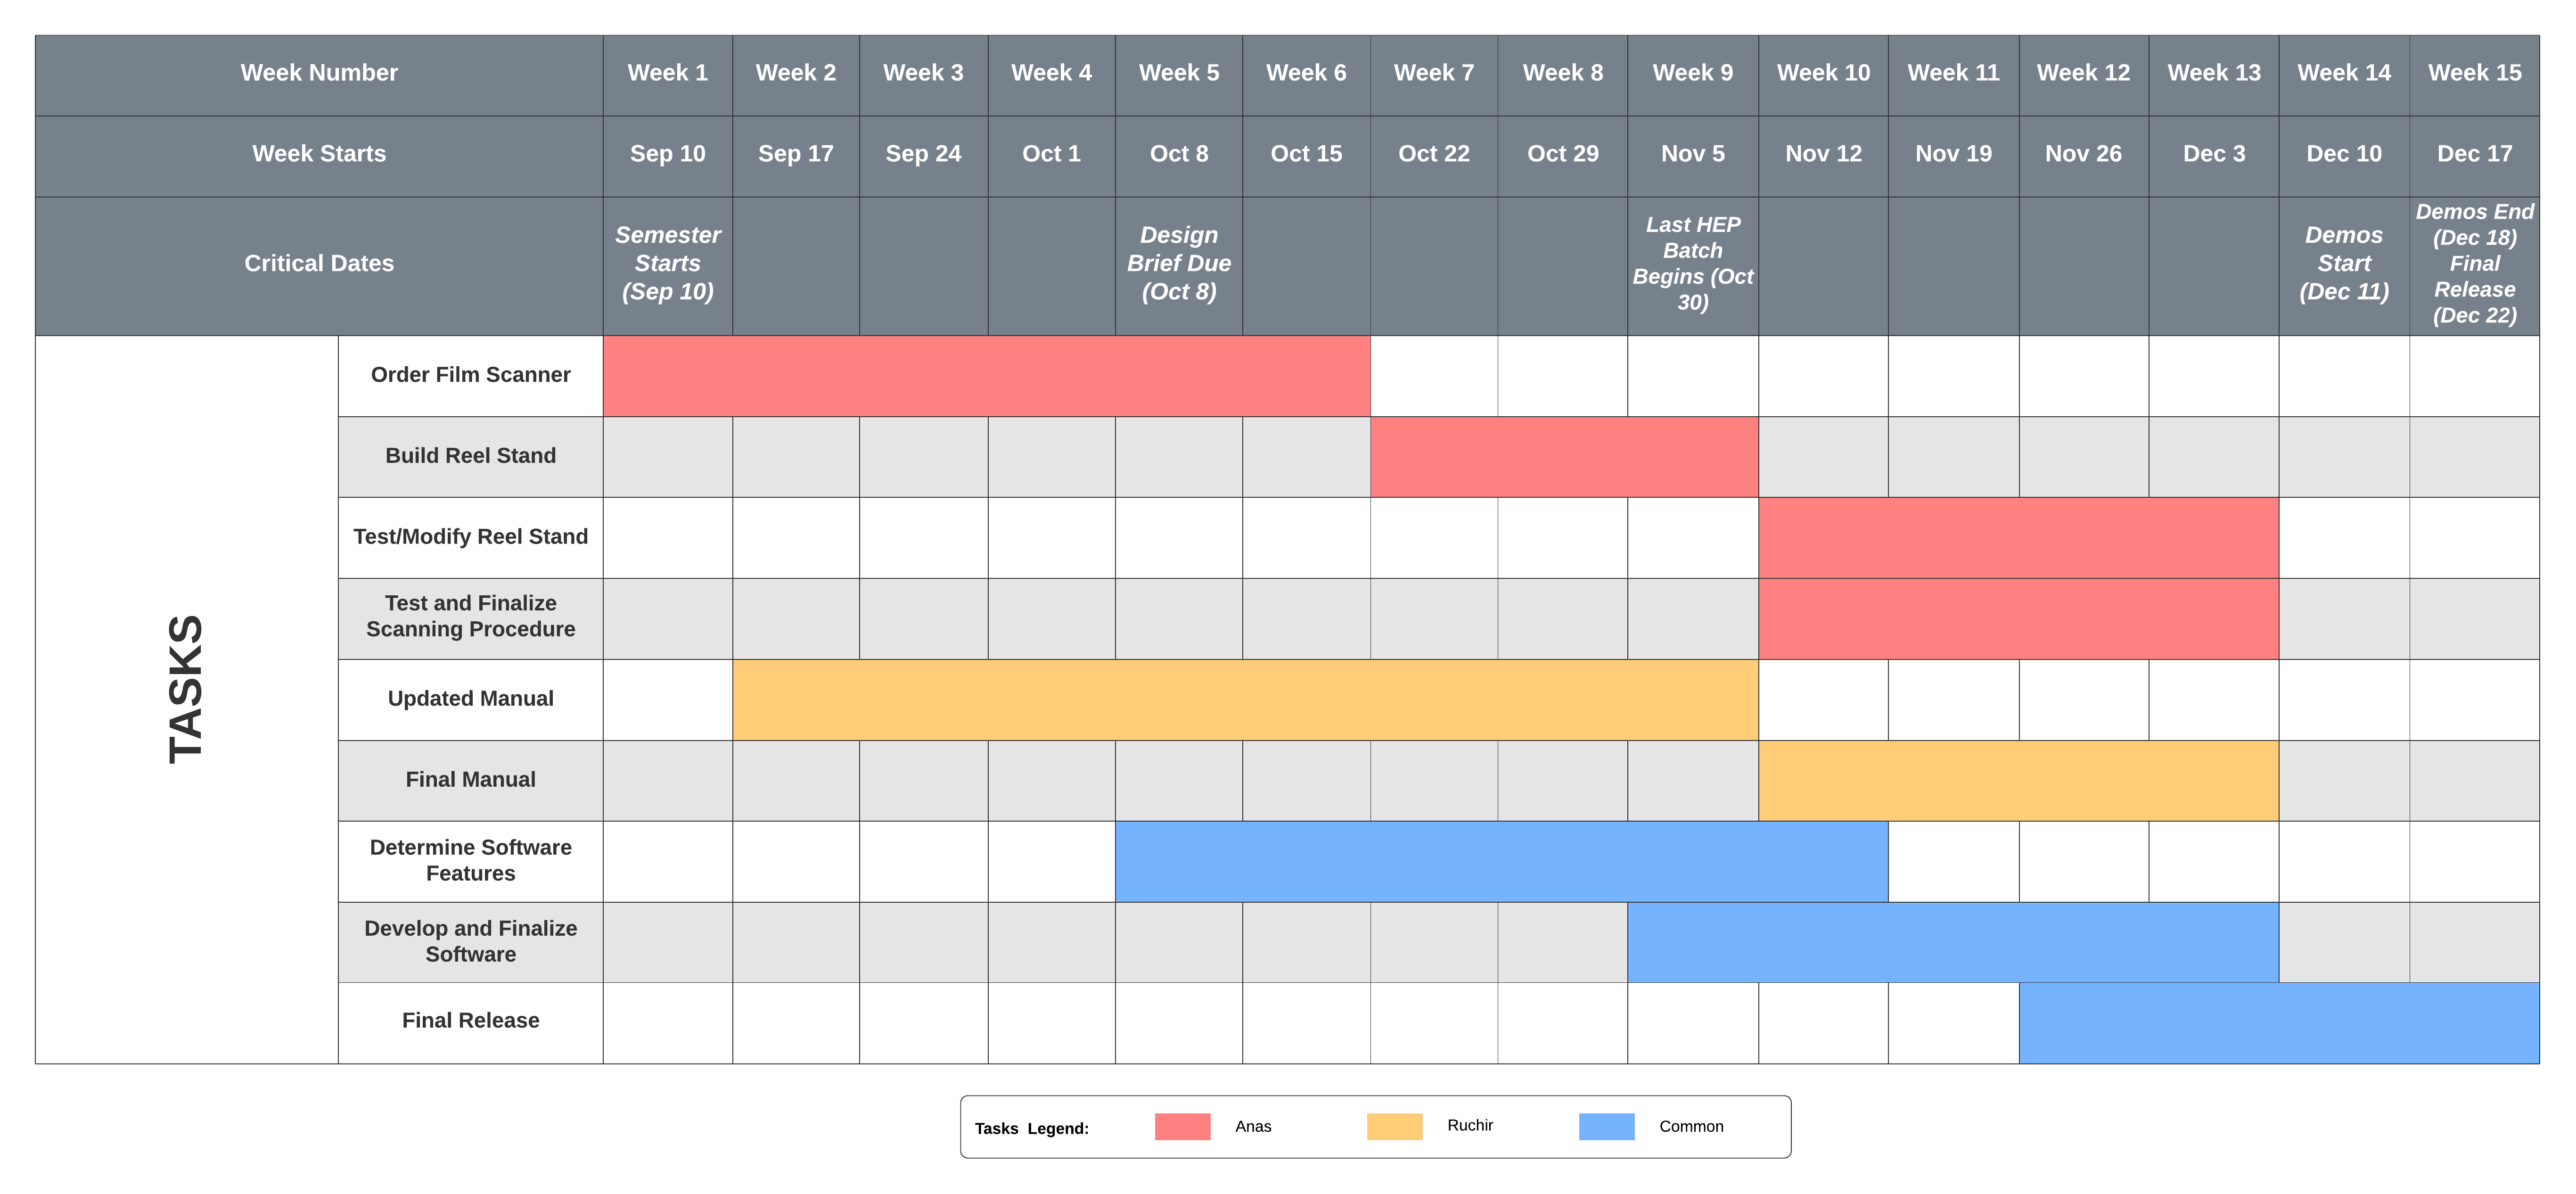
\includegraphics[width = 1.0\linewidth]{Images/Gantt chart - HEP.png} 
    \caption{GANTT Chart for HEP Capstone Project. Respective tasks are shown to span over several weeks at a time as shown by the coloured bars.}
    \label{fig: gantt}
\end{SidewaysFigure}

\begin{SidewaysFigure}
    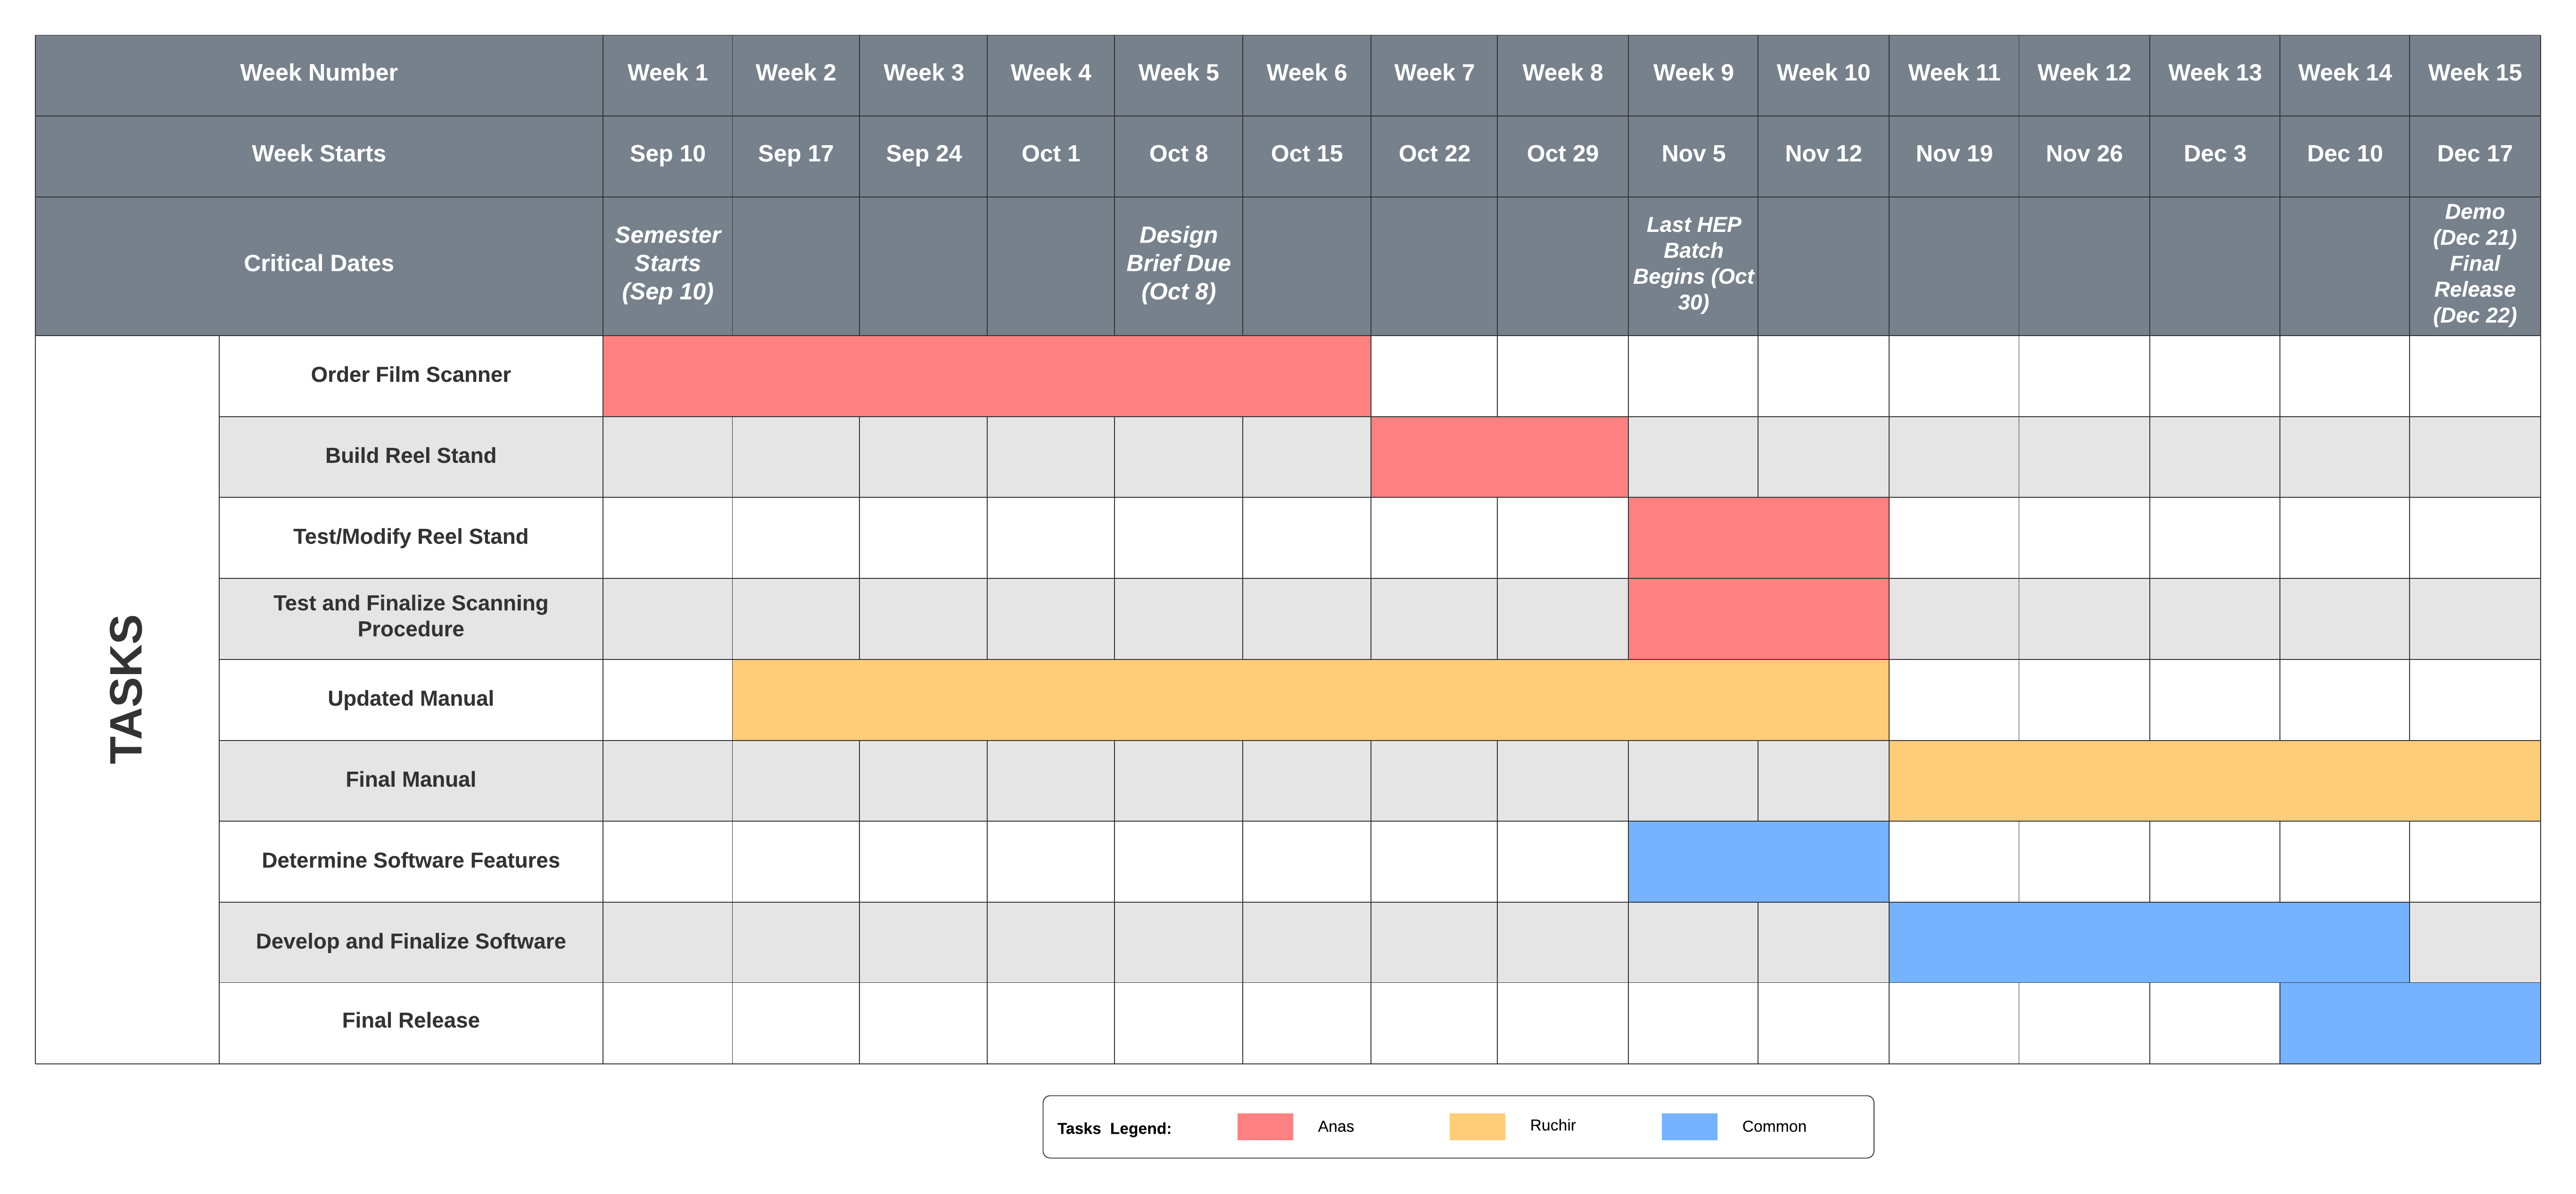
\includegraphics[width = 1.0\linewidth]{Images/Final Gantt chart - HEP.png} 
    \caption{Final GANTT Chart for HEP Capstone Project. Respective tasks are shown to span over several weeks at a time as shown by the coloured bars.}
    \label{fig: final_gantt}
\end{SidewaysFigure}

In figure \ref{fig: gantt} and figure \ref{fig: final_gantt}, ``Updated Manual" refers to the the updated manual for the current version of the HEP experiment, without the new software features. ``Final Manual" thus refers to the final version of the manual which included instructions on using all final features of the software. As the third and final experiments of the Advanced Lab began on October 30, the actual due date for the Updated manual was October 29 (we had initially planned for at least one set of student experimenters to test out the manual, however as we will see below this was not possible).

Ultimately, we decided not to purchase a new scanner for the project, so the time spent researching different scanning options may be considered ``wasted". However, this decision was made mainly because all other options had been considered and using the Advanced Lab's Epson Perfection 4990 Photo was the best. Knowledge of film scanning also helped greatly in reel stand testing. The knowledge gained through this project will also help inform future decisions made by the Advanced Physics Lab regarding the film scanner. Thus, we were somewhat successful at following our initial timeline with regard to the ordering of the film scanner. 

Building and testing the reel stands took much less time than initially expected, mainly due to improvements in the reel stands' design, their construction was made much simpler. Testing was also much easier that expected due to knowledge of film scanning we gained from researching all the different scanning options. Thus, we were quite successful at following our initial timeline with regard to the building and testing of the reel stand. 

Initially, we had planned to provide the last batch of HEP students with an updated version of the manual so that they could use it and provide us with feedback. We met our deadlines for the finishing the manual in time to allow this, but the manual was not forwarded to the students in time for them to provide feedback. However, we got valuable feedback from Professor Bailey and other instructors of the HEP lab, so we were overall successful in receiving feedback in a timely manner. The manual was written in such a way that it would be easily comprehensible for undergraduates, and more readable than the previous version of the manual. Thus, we were generally successful at following our initial timeline with regard to the manual. 

Due to our somewhat late start to the development of the additional  software features in Traxis, no student experimenters got the chance to test out the additional features. As seen in figure \ref{fig: gantt}, the engineering design team had not initially planned for student experimenters to test out the features due to time constraints. This proved to be true, as seen in figure \ref{fig: final_gantt}, as the software development time exceeded our initial prediction. However, the engineering design team was able to use their own experience as former HEP lab students as a proxy for the experience of current HEP lab students; hence, features were designed to be intuitive to use. Thus, we were generally successful at following our initial timeline with regard to the development of the software. 

\subsection{Budget}
The budget for this project was controlled by Professor Bailey. While Professor Bailey did not declared any single budget value, he provided a vague estimate for a maximum reasonable price for a film scanner, which was around \$2000. Moreover, he did not estimate a budget for the development of the reel stands as they were expected to cost only around \$100 to construct. Of course, writing the manual and expanding the software was expected to be free, which turned out to be true. Overall, Professor Bailey had expressed that the budget was fluid if we could justify our spending with a well done project.

We did not need to purchase a new scanner as the Epson Perfection 4990 Photo present in the Advanced Lab was selected for use. Moreover, the reel stands costed a total of \$80. Therefore, the project was overall well within budget. There were also no surprise expenses as all costs had been anticipated during initial budgeting.

\newpage

\bibliographystyle{ieeetr}
\bibliography{bib}


\end{document}
